%!TEX root = ../dokumentation.tex

\chapter{Training von Klassifikationsmodellen} \label{ch:crispDm_2}

Auf Basis der bereinigten Datensätze werden im folgenden Abschnitt diverse Klassifikationsmodelle trainiert. Dies umfasst Baseline-Modelle mit \ac{BoW} und \ac{TF-IDF}, als auch neuronale Netze, die zusätzlich auf komprimierten Worteinbettungen trainiert werden. Ferner wird mit \ft und \ac{BERT} Modellen trainiert.

Grundlegend wird jedes Modell separat auf jedem Datensatz (Tweets, Reden, Wahlprogramme) trainiert. Im Folgenden wird diese Methode als \textit{in-domain} referenziert. Modelle, die es durch ihren Ressourcenbedarf (Speicher und Rechenkapazität) zulassen, werden ebenfalls auf dem kombinierten Datensatz trainiert. 

Wie \autoref{tab:countPerDatasetAfterCleaning} zeigt, sind die Klassen innerhalb der einzelnen Datensätze nicht ausgeglichen. Dies kann zu einem Bias hin zur am stärksten vertretenen Klasse führen. Zusätzlich zu den unbalancierten Daten werden die Klassen der Datensätze ebenfalls mit Unterabtastung (engl. undersampling) angeglichen. Als Metrik wird der Makro \(F_1\) Score verwendet. Dieser ergibt sich aus dem ungewichteten Durchschnitt der \(F_1\) Werte aller Klassen. Diese Metrik wird gewählt, um die Performance für jede Partei gleich zu gewichten, unabhängig von der Anzahl an Einträgen pro Partei.

Für das Training der Baseline-Modelle sowie neuronalen Netze steht ein MacBook Pro mit dem Apple M1 Pro Prozessor und \num{8} Kernen zur Verfügung. Zudem bietet das MacBook \SI{16}{\giga\byte} an \ac{RAM} und eine \ac{GPU} mit \num{14} Kernen. Jegliche Trainings mit \ft oder \ac{BERT} erfolgen auf einem Computer mit einer Intel Xeon E3-1231 v3 \ac{CPU} mit \num{4} Kernen und \num{8} Threads. Außerdem verfügt der Computer über \SI{16}{\giga\byte} an \ac{RAM} und einer Nvidia GeForce GTX 1070 mit \SI{8}{\giga\byte} an \ac{GDDR5} Speicher.

\section{Baseline} \label{sec:trainingBaseline}

Als ersten Ansatz zum Training eines Klassifikationsmodells werden -- als \enquote{Baseline} -- simple \ac{ML}-Verfahren auf der Basis von kontextunabhängigen Textrepräsentationsformen verwendet. Dabei werden die Trainings-Daten in Form von Text zuerst mittels \ac{BoW} als auch \ac{TF-IDF} vektorisiert, um als Input für ein Klassifikationsverfahren genutzt werden zu können.

Die Transformation der Eingabedaten resultiert in einer Matrix der Größe \(N \times V\), mit \(N\) als Anzahl der Datenpunkte und \(V\) der Größe des Vokabulars beziehungsweise der Anzahl aller einzigartigen Wörter im gesamten Datensatz. Das Vokabular wird im Folgenden auf die \num{50000} im Datensatz am meisten vorkommenden Wörter begrenzt. Dadurch wird vermieden, dass die Matrix zu groß wird und der \ac{RAM} auf dem genutzten Computer nicht ausreicht. Die zweite Dimension, die Anzahl an Einträgen eines Datensatzes, muss für die Tweets auf \num{125000} begrenzt werden. Bei der Beurteilung der Ergebnisse sollte berücksichtigt werden, dass daher nur gut ein Drittel der zur Verfügung stehenden Tweets bei auf \ac{BoW} oder \ac{TF-IDF} basierenden Ansätzen zum Training verwendet werden kann.

Bei der Umwandlung von Text zu Vektoren werden nur Wörter miteinbezogen, die in maximal \SI{20}{\percent} der Einträge vorkommen (\(max\_df = \num{0.2}\)). Das Ziel dabei ist, generische Wörter aus den Datensätzen zu filtern. Somit werden ausschließlich Wörter berücksichtigt, die eine besondere Aussage haben und als repräsentativ für die jeweilige Partei anzusehen sind. Die Python-Bibliothek \sk, die für die Vektorisierung und das Trainieren der Baseline-Modelle verwendet wird, bietet ebenfalls die Möglichkeit, nicht nur einzelne Wörter (1-grams) zur Repräsentation zu nutzen, sondern beliebige n-grams. Diese Option wird nicht genutzt (\(ngram\_range = (\num{1}, \num{1})\)), weil -- wie bereits angesprochen -- die Dimension der transformierten Matrix sonst zu groß werden würde. Außerdem stellt \ft eine ähnliche Methode bereit.

\sk~bietet eine Reihe von Klassifikations-Algorithmen, die zusätzlich zur binären Klassifikation ebenfalls mehrere Klassen unterstützt \autocite{noauthor_112_nodate}. Hervorgehend aus den Experimenten erreichen Multinomial \ac{NB} sowie Lineare \ac{SVC} die beste Performance. Andere Modelle erreichen einen deutlich geringeren \(F_1\) Score\footnote{\texttt{KNeighborsClassifier}, \texttt{DecisionTreeClassifier} und \texttt{ExtraTreeClassifier}} oder trainieren wesentlich länger\footnote{\texttt{LogisticRegression}, \texttt{GradientBoostingClassifier} und \texttt{RandomForestClassifier}}.

Für die beiden gewählten Modelle sowie die Vektorisierung durch \ac{BoW} und \ac{TF-IDF} wird eine Hyperparameteroptimierung durch eine Rastersuche in \sk~ausgehend von den Standardparametern durchgeführt. Dadurch ergibt sich eine Erhöhung der maximal durchzuführenden Iterationen bei der Linearen \ac{SVC} (\(max\_iter = \num{2000}\)) sowie die bereits dargestellte Konfiguration der Vektorisierung. Als Eingabetext wird jeweils der auf die Wortstämme reduzierte und tokenisierte Text verwendet.
    
{\footnotesize
\begin{longtblr}[caption={Macro \(F_1\) Score für Lineare \acs{SVC}}, label={tab:overviewScoresBaselineSvc}, note{$\dag$}={Aufgrund von beschränkten Rechenressourcen zum Training wird der Datensatz auf \num{125000} zufällig ausgewählte Einträge beschränkt.}, remark{Parameter} = {\(max\_df = \num{0.2}\), \(ngram\_range = (\num{1}, \num{1})\), \(max\_iter = \num{2000}\)}]{hline{1, 3, Z} = {0.75pt}, rowhead = 2, colspec={l*{4}{Q[si={table-format=1.2},c]}}, row{1-2}={guard,font=\bfseries,l}}
     & \SetCell[c=2]{c} BoW & & \SetCell[c=2]{c} TF-IDF & \\
    \cline{2-5}
    Datensatz & Unbalanced & Balanced & Unbalanced & Balanced \\

    Tweets\TblrNote{$\dag$} & 0.50 & 0.49 & \textbf{\num{0.54}} & 0.52 \\*
    Wahlprogramme & 0.50 & 0.47 & \textbf{\num{0.55}} & 0.51 \\*
    Reden & 0.62 & 0.59 & \textbf{\num{0.66}} & 0.63 \\
\end{longtblr}
}

Lineare \acp{SVC} lassen sich sehr schnell trainieren. Je nach Datensatz beträgt die Dauer \SI{20}{\second} bis \SI{3}{\minute}.

\autoref{tab:overviewScoresBaselineSvc} stellt die Ergebnisse des Trainings der Linearen \ac{SVC} auf allen drei Datensätzen einzeln und je auf Basis von \ac{BoW} und \ac{TF-IDF} dar. Als Metrik dient der Makro \(F_1\) Score. Das Training wurde sowohl auf dem unbalancierten (\enquote{unbalanced}) als auch auf einem durch Undersampling balancierten Datensatz mit gleicher Verteilung der Klassen (\enquote{balanced}) durchgeführt.

Auf jedem Datensatz erreicht \ac{TF-IDF} den höchsten \(F_1\) Score. Der Tweet-Datensatz erreicht mit \num{0.54}, knapp hinter den Wahlprogrammen mit \num{0.55}, den schlechtesten Wert. Das Training auf den Reden erreicht einen deutlich bessere Score von \num{0.66}. Das Balancieren der Datensätze senkt das Ergebnis jeweils um \numrange{0.2}{0.04}. \ac{BoW} schneidet konstant um \numrange{0.03}{0.05} Punkte schlechter ab als \ac{TF-IDF}.

{\footnotesize
\begin{longtblr}[caption={Makro \(F_1\) Score für Multinomial \acs{NB}}, label={tab:overviewScoresBaselineNb}, note{$\dag$}={Aufgrund von beschränkten Rechenressourcen zum Training wird der Datensatz auf \num{125000} zufällig ausgewählte Einträge beschränkt.}, remark{Parameter} = {\(max\_df = \num{0.2}\), \(ngram\_range = (\num{1}, \num{1})\)}]{hline{1, 3, Z} = {0.75pt}, rowhead = 2, colspec={l*{4}{Q[si={table-format=1.2},c]}}, row{1-2}={guard,font=\bfseries,l}}
     & \SetCell[c=2]{c} BoW & & \SetCell[c=2]{c} TF-IDF & \\
    \cline{2-5}
    Datensatz & Unbalanced & Balanced & Unbalanced & Balanced \\

    Tweets\TblrNote{$\dag$} & \textbf{\num{0.53}} & 0.52 & 0.52 & 0.51 \\*
    Wahlprogramme & \textbf{\num{0.51}} & 0.49 & 0.24 & 0.50 \\*
    Reden & \textbf{\num{0.61}} & 0.60 & 0.14 & 0.60 \\
\end{longtblr}
}

Das Training von Multinomial \ac{NB} dauert ebenfalls nicht lange. Je nach Datensatz beträgt die Trainingsdauer \SI{10}{\second} bis \SI{8}{\minute}.

Die gleichen Trainings werden zudem mit Multinomial \ac{NB} durchgeführt. Dazu stellt \autoref{tab:overviewScoresBaselineNb} die Ergebnisse in gleicher Form dar. Anders als zuvor führt die Text-Vektorisierung mittels \ac{BoW} bei allen Datensätzen zu dem besten \(F_1\) Score. Die Wahlprogramme erreichen mit \num{0.51} den geringsten Wert. Der Tweet-Datensatz erreicht \num{0.53} und die Reden liefern mit \num{0.61} das beste Ergebnis. Auf balancierten Daten schneidet \ac{BoW} leicht schlechter ab. Mit \ac{TF-IDF} lässt sich für die unbalancierten Tweets ein ähnlich hoher \(F_1\) Score von \num{0.52} erreicht. Im Gegensatz zu \ac{BoW} fällt dieser für die unbalancierten Wahlprogramme und Reden aber auf \numrange{0.14}{0.24}. Auf den balancierten Datensätzen tritt diese Anomalie nicht auf. \ac{BoW} und \ac{TF-IDF} erreichen auf diesen nahezu identische Werte.

Die in \autoref{tab:overviewScoresBaselineSvc} und \autoref{tab:overviewScoresBaselineNb} dargestellten Ergebnisse betrachten jeweils mit dem Makro \(F_1\) Score einen gewichteten Durchschnitt zwischen den Ergebnissen für die einzelnen klassifizierten Parteien. Im Folgenden soll anhand der in \autoref{fig:confusionMatrixBaseline} dargestellten Konfusionsmatrizen genauer untersucht werden, welche Parteien besonders gut erkannt werden können und zwischen welchen Parteien viele Verwechslungen auftreten. Dabei wird auf die Ergebnisse des besten Baseline-Modells, der Linearen \ac{SVC} mit \ac{TF-IDF}, zurückgegriffen.

\begin{figure}[H]
    \centering
    \begin{subfigure}{0.49\textwidth}
        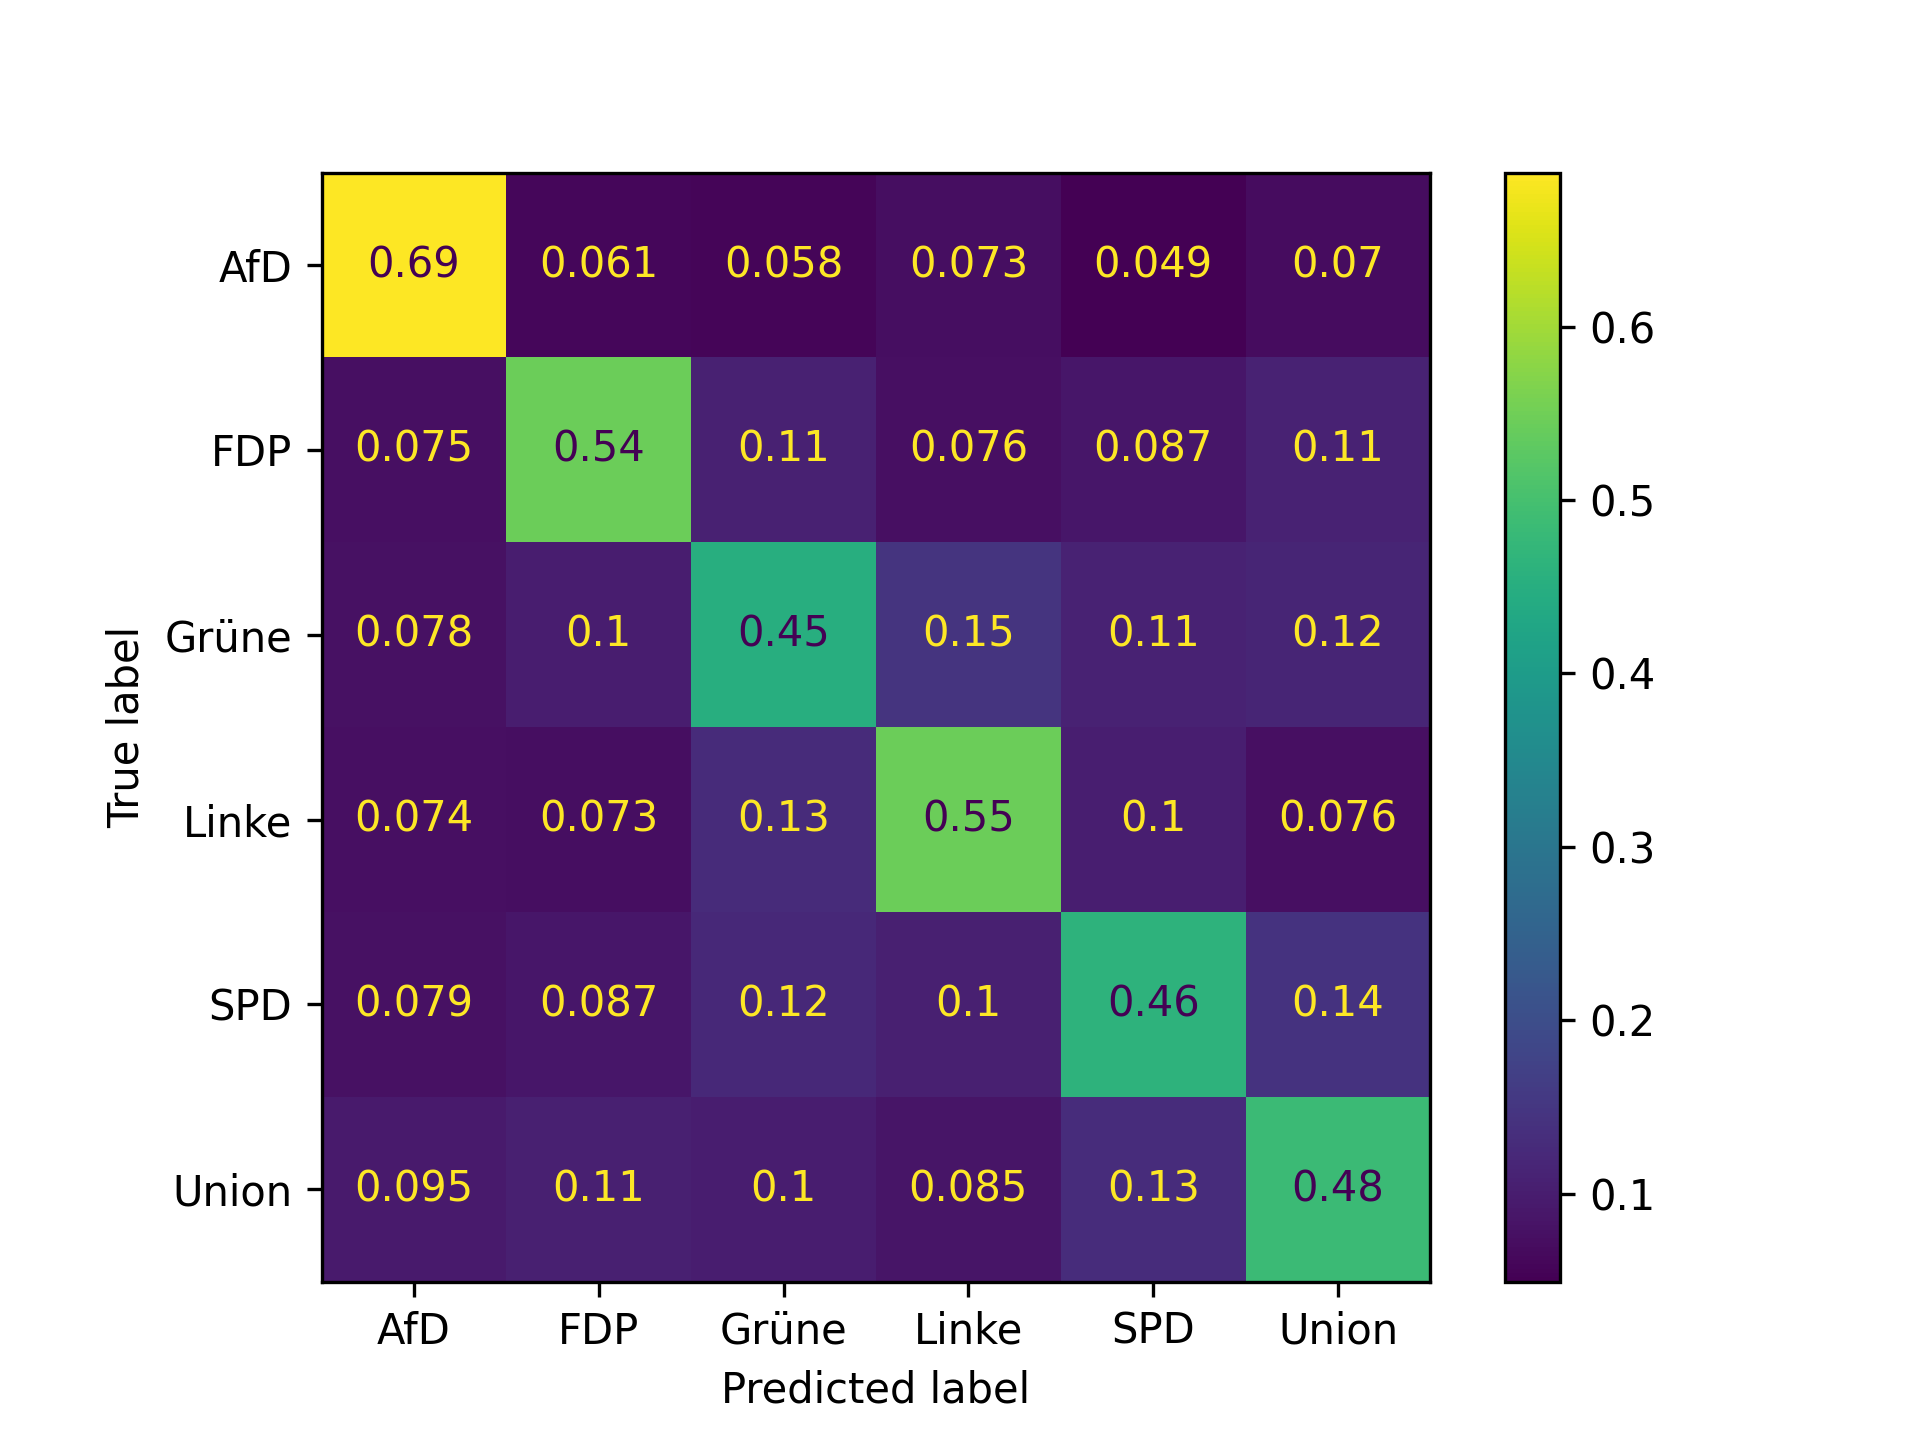
\includegraphics[width=\textwidth]{data/images/modeling/baseline/under/tweets_confusion_matrix.png}
        \caption{Tweets}
        \label{sfig:confusionMatrixBaselineTweets}
    \end{subfigure}
    \hfill
    \begin{subfigure}{0.49\textwidth}
        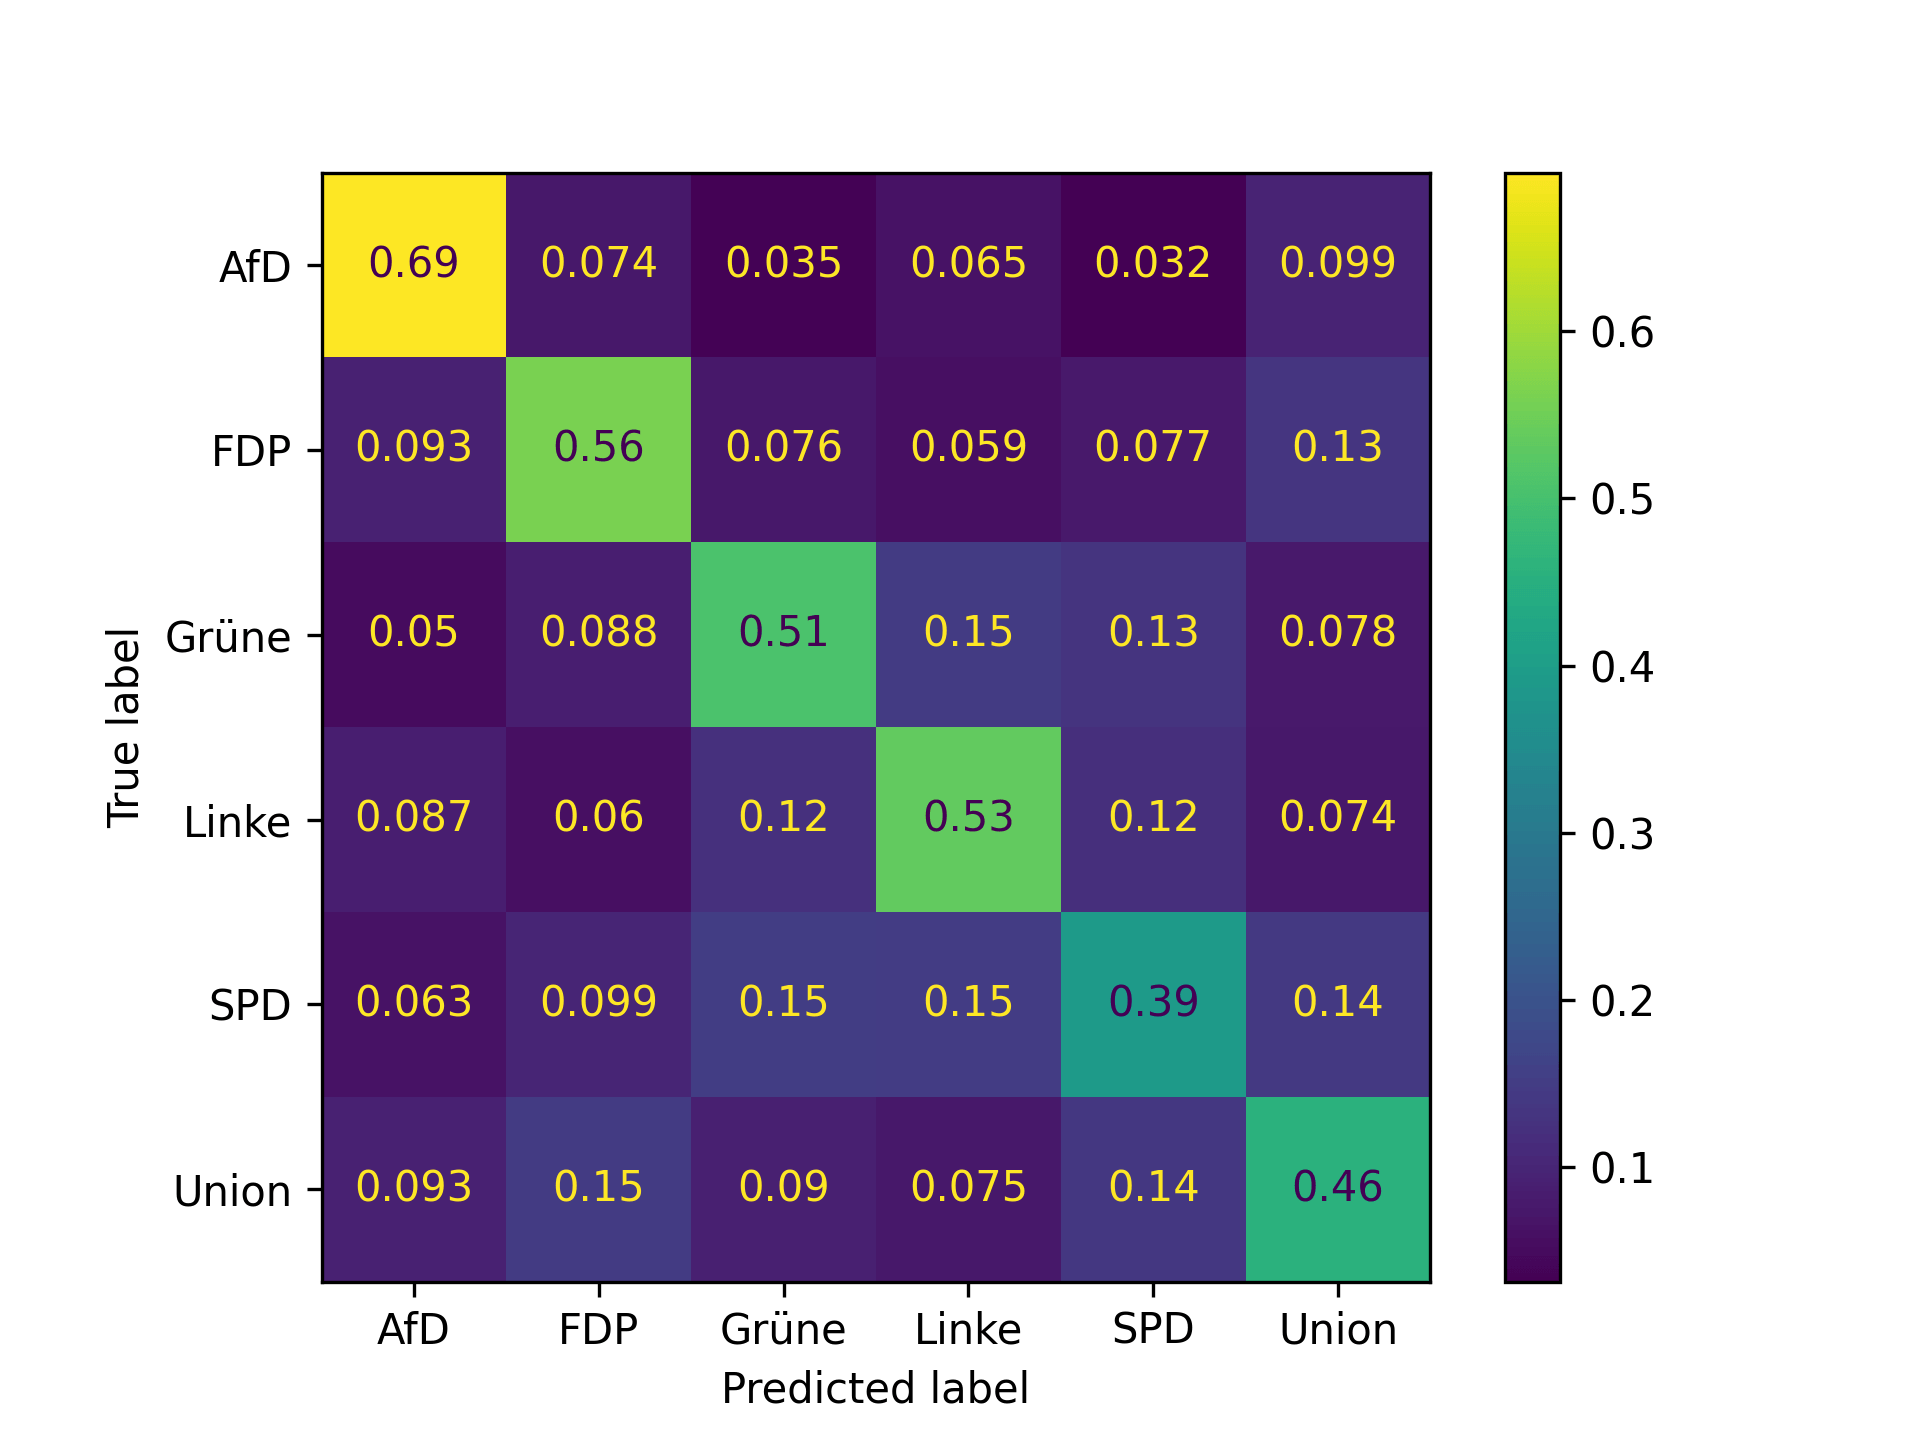
\includegraphics[width=\textwidth]{data/images/modeling/baseline/under/party_programs_confusion_matrix.png}
        \caption{Wahlprogramme}
        \label{sfig:confusionMatrixBaselineManifest}
    \end{subfigure}
    \hfill
    \begin{subfigure}{0.49\textwidth}
        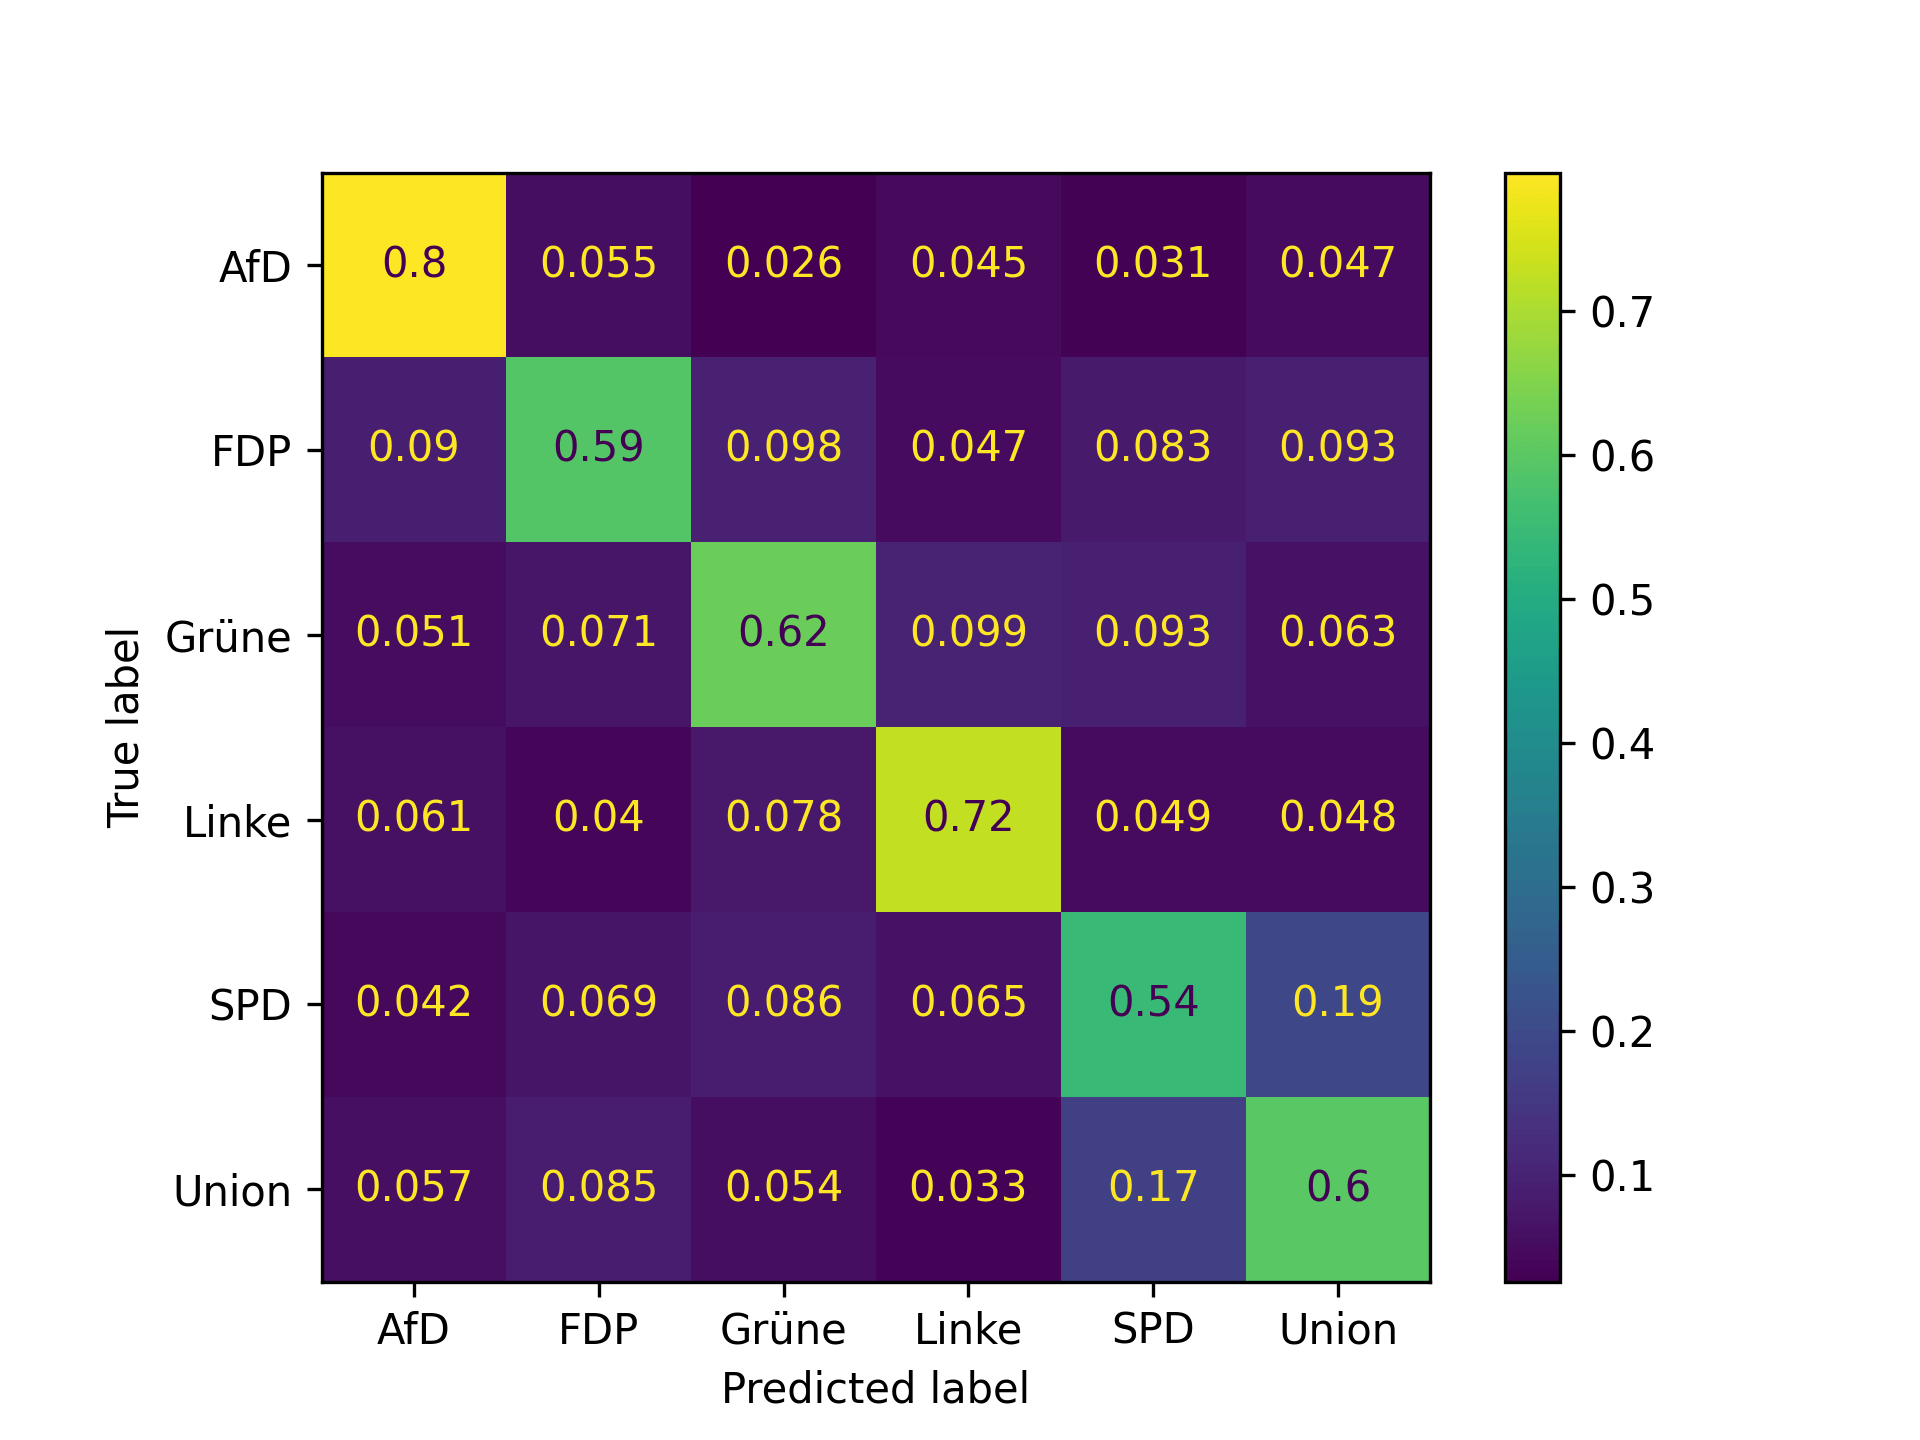
\includegraphics[width=\textwidth]{data/images/modeling/baseline/under/speeches_confusion_matrix.png}
        \caption{Reden}
        \label{sfig:confusionMatrixBaselineSpeeches}
    \end{subfigure}
    \caption{Konfusionsmatrizen für Lineare \acs{SVC} mit \acs{TF-IDF} auf ausgeglichenen Datensätzen} \label{fig:confusionMatrixBaseline}
\end{figure}

Bei den Tweets (\autoref{sfig:confusionMatrixBaselineTweets}) lässt sich die \ac{AfD} am besten klassifizieren. Unter allen Tweets, die als \ac{AfD} klassifiziert wurden, sind \SI{69}{\percent} korrekt klassifiziert. Die Matrix zeigt keine Partei, die besonders häufig mit der \ac{AfD} verwechselt wurde. Am zweitbesten, mit \SI{55}{\percent}, erkennt das Modell Tweets der Linken. Am häufigsten wird die Linke mit den anderen beiden Parteien im linken Spektrum verwechselt. So werden zu \SI{13}{\percent} Tweets der Linken den Grünen und \SI{10}{\percent} der \ac{SPD} zugeordnet. Bei den Grünen treten viele Verwechslungen zu allen Parteien außer der \ac{AfD} auf. Bei den Tweets der \ac{SPD} kommt zu Grünen und Linken die Union hinzu. Die Tweets der Union selbst werden zu \SI{13}{\percent} als \ac{SPD} klassifiziert. Tweets der \ac{FDP} werden zu jeweils \SI{11}{\percent} den Grünen und der Union zugeordnet. Allgemein ist festzuhalten, dass Tweets einer politischen Partei häufig als politisch nahestehende Partei klassifiziert werden. Weiterhin ist festzustellen, dass die Falsch-Positiv- und Falsch-Negativ-Raten in \autoref{sfig:confusionMatrixBaselineTweets} symmetrisch entlang Richtig-Positiv Achse auftreten.

Die \autoref{sfig:confusionMatrixBaselineManifest} zeigt die Konfusionsmatrix für die Wahlprogramme. Parteien, die sich politisch nahe stehen, weisen ebenfalls wie bei den Tweets eine höhere Falsch-Negativ-Rate auf. Auffällig ist, dass die Falsch-Negativ-Rate bei der \ac{SPD} und der Union deutlich höher ist als bei den anderen Parteien. Die beiden Regierungsparteien erreichen eine Richtig-Positiv-Rate von \SIrange{39}{46}{\percent}, während die Oppositionsparteien bei \SIrange{51}{69}{\percent} liegen. Die Konfusionsmatrix weist ebenfalls wie \autoref{sfig:confusionMatrixBaselineTweets} eine Symmetrie entlang der Richtig-Positiv Achse auf.

Der Datensatz der Reden führt insgesamt zu der höchsten Genauigkeit. Die Konfusionsmatrix \autoref{sfig:confusionMatrixBaselineSpeeches} zeigt, dass die Reden der \ac{AfD} mit \SI{80}{\percent} und der Linken mit \SI{72}{\percent} am besten klassifiziert werden. Die Reden der anderen Parteien erreichen für die Richtig-Positiv-Rate lediglich zwischen \SIrange{54}{62}{\percent}. Grundsätzlich weist die Konfusionsmatrix für die Reden wenige Übereinstimmungen mit den anderen beiden Matrizen im allgemeinen Muster auf. Die stärkste Verwechslung über alle Datensätze hinweg tritt bei Reden der \ac{SPD} auf. Diese werden zu \SI{19}{\percent} als Reden der Union klassifiziert. Die Reden der Union werden ebenfalls zu \SI{17}{\percent} der \ac{SPD} zugeordnet. 

Bei allen drei Konfusionsmatrizen weisen die \ac{SPD} und \ac{CDU} eine starke gegenseitige Verwechselung auf. Ein weiterer Faktor, neben der politischen Nähe, könnte sein, dass die beiden Parteien im Untersuchungszeitraum zusammen die Regierung gebildet haben.

\section{fastText} \label{sec:trainingFastText}

\ft ist eine Methode zum Generieren von Worteinbettungen, die von Facebook Research entwickelt wurde \autocite{joulin_bag_2016}. Wie schon in \autoref{sec:representationForms} dargelegt, basiert die Methodik darauf, Wörter in n-grams zu zerlegen. Resultierend lassen sich auch Wörter klassifizieren, die nicht im Trainingsdatensatz für die Worteinbettungen enthalten waren \autocite{guhr_training_2020}. Auf den sich ergebenden Worteinbettungen kann schließlich ein Klassifikator trainiert werden.

Für das folgende Training wird die \texttt{fastText}\footnote{\href{https://pypi.org/project/fasttext/}{https://pypi.org/project/fasttext/}} Bibliothek für Python verwendet. Um die Worteinbettungen von \ft zu nutzen, ist es möglich entweder eigenständig die Einbettungen zu trainieren oder vortrainierte Einbettungen zu verwenden. Im Rahmen dieser Arbeit werden vortrainierte Einbettungen\footnote{\href{https://fasttext.cc/docs/en/crawl-vectors.html}{https://fasttext.cc/docs/en/crawl-vectors.html}} verwendet, da die eigene Erstellung solcher Einbettungen eine große Menge an Daten benötigt. Die vortrainierten, deutschen Worteinbettungen basieren auf dem Common Crawl\footnote{\href{https://commoncrawl.org/}{https://commoncrawl.org/}} und Wikipedia\footnote{\href{https://www.wikipedia.org/}{https://www.wikipedia.org/}} Datensatz.

Für das Training werden die Hyperparameter von \textcite{guhr_training_2020} übernommen. Demnach wird mit allen Einträgen pro Datensatz für \num{20} Epochen und einer Lernrate von \num{0.1} trainiert. Für das Training werden einerseits wie bei \citeauthor{guhr_training_2020} Bigramme und andererseits zusätzlich auch Trigramme verwendet. Im Gegensatz zu \textcite{guhr_training_2020} kommen im Folgenden die zuvor beschriebenen, vortrainierte Worteinbettungen mit einer Vektorgröße von \num{300} zum Einsatz.

{\footnotesize
\begin{longtblr}[caption={Makro \(F_1\) Score für \ft}, label={tab:overviewScoresFastText}, remark{Parameter} = {\(E = \num{20}\), \(LR_{init} = \num{0.1}\)}]{hline{1, 3, Y-Z} = {0.75pt}, rowhead = 2, colspec={l*{4}{Q[si={table-format=1.2},c]}}, row{1-2}={guard,font=\bfseries,l}}
     & \SetCell[c=2]{c} Bigramme (\(n = \num{2}\)) & & \SetCell[c=2]{c} Trigramme (\(n = \num{3}\)) & \\ 
    \cline{2-5}
    Datensatz & Unbalanced & Balanced & Unbalanced & Balanced \\ 

    Tweets & \textbf{\num{0.59}} & 0.58 & \textbf{\num{0.59}} & 0.57 \\*
    Wahlprogramm & \textbf{\num{0.58}} & 0.54 & 0.57 & 0.54 \\*
    Reden & \textbf{\num{0.69}} & 0.65 & 0.67 & 0.66 \\*
    
    Kombiniert & \textbf{\num{0.59}} & 0.57 & 0.58 & 0.57 \\
\end{longtblr}
}

\ft lässt sich rasch trainieren. Insgesamt, mit dem Laden der Daten, benötigt das Trainieren circa \SI{2}{\minute}, wovon das reine Training knapp \SI{30}{\second} ausmacht.

\autoref{tab:overviewScoresFastText} zeigt die Makro \(F_1\) Scores, die mittels \ft erreicht werden. Aus den Ergebnissen geht hervor, dass durchweg das Training auf den unbalancierten Datensätzen zu höheren \(F_{1}\) Scores führt. Auf den unbalancierten Daten mit Bigrammen erreichen Tweets und Wahlprogramme einen \(F_{1}\) von \numrange{0.58}{0.59}. Den höchsten Wert erreichen die Reden mit \num{0.69}. Auf den balancierten Daten schneiden die Bigramme zwischen \numrange{0.01}{0.04} schlechter ab. Trigramme erreichen lediglich auf den unbalancierten Tweets den identischen Score wie Bigramme. Die unbalancierten Wahlprogramme und Reden schneiden jeweils \num{0.02} schlechter ab. Auf den balancierten Wahlprogrammen erreichen Trigramme ebenfalls den gleichen Wert, während balancierte Tweets und Reden jeweils um \num{0.01} schlechter abschneiden.

Auf den kombinierten, unbalancierten Daten erreichen die Bigramme einen Makro \(F_1\) Score von \num{0.59}. Den insgesamt zweitbesten Wert erreichen die Trigramme auf ebenfalls unbalancierten Daten. Auf balancierten Daten erreichen Bi- und Trigramme einen Wert von \num{0.57}.

Um einen Bias durch unbalancierte Daten zu vermeiden, wird das \ft Modell auf Bigrammen und den balancierten Daten präferiert.

\begin{figure}[H]
    \centering
    \begin{subfigure}{0.49\textwidth}
      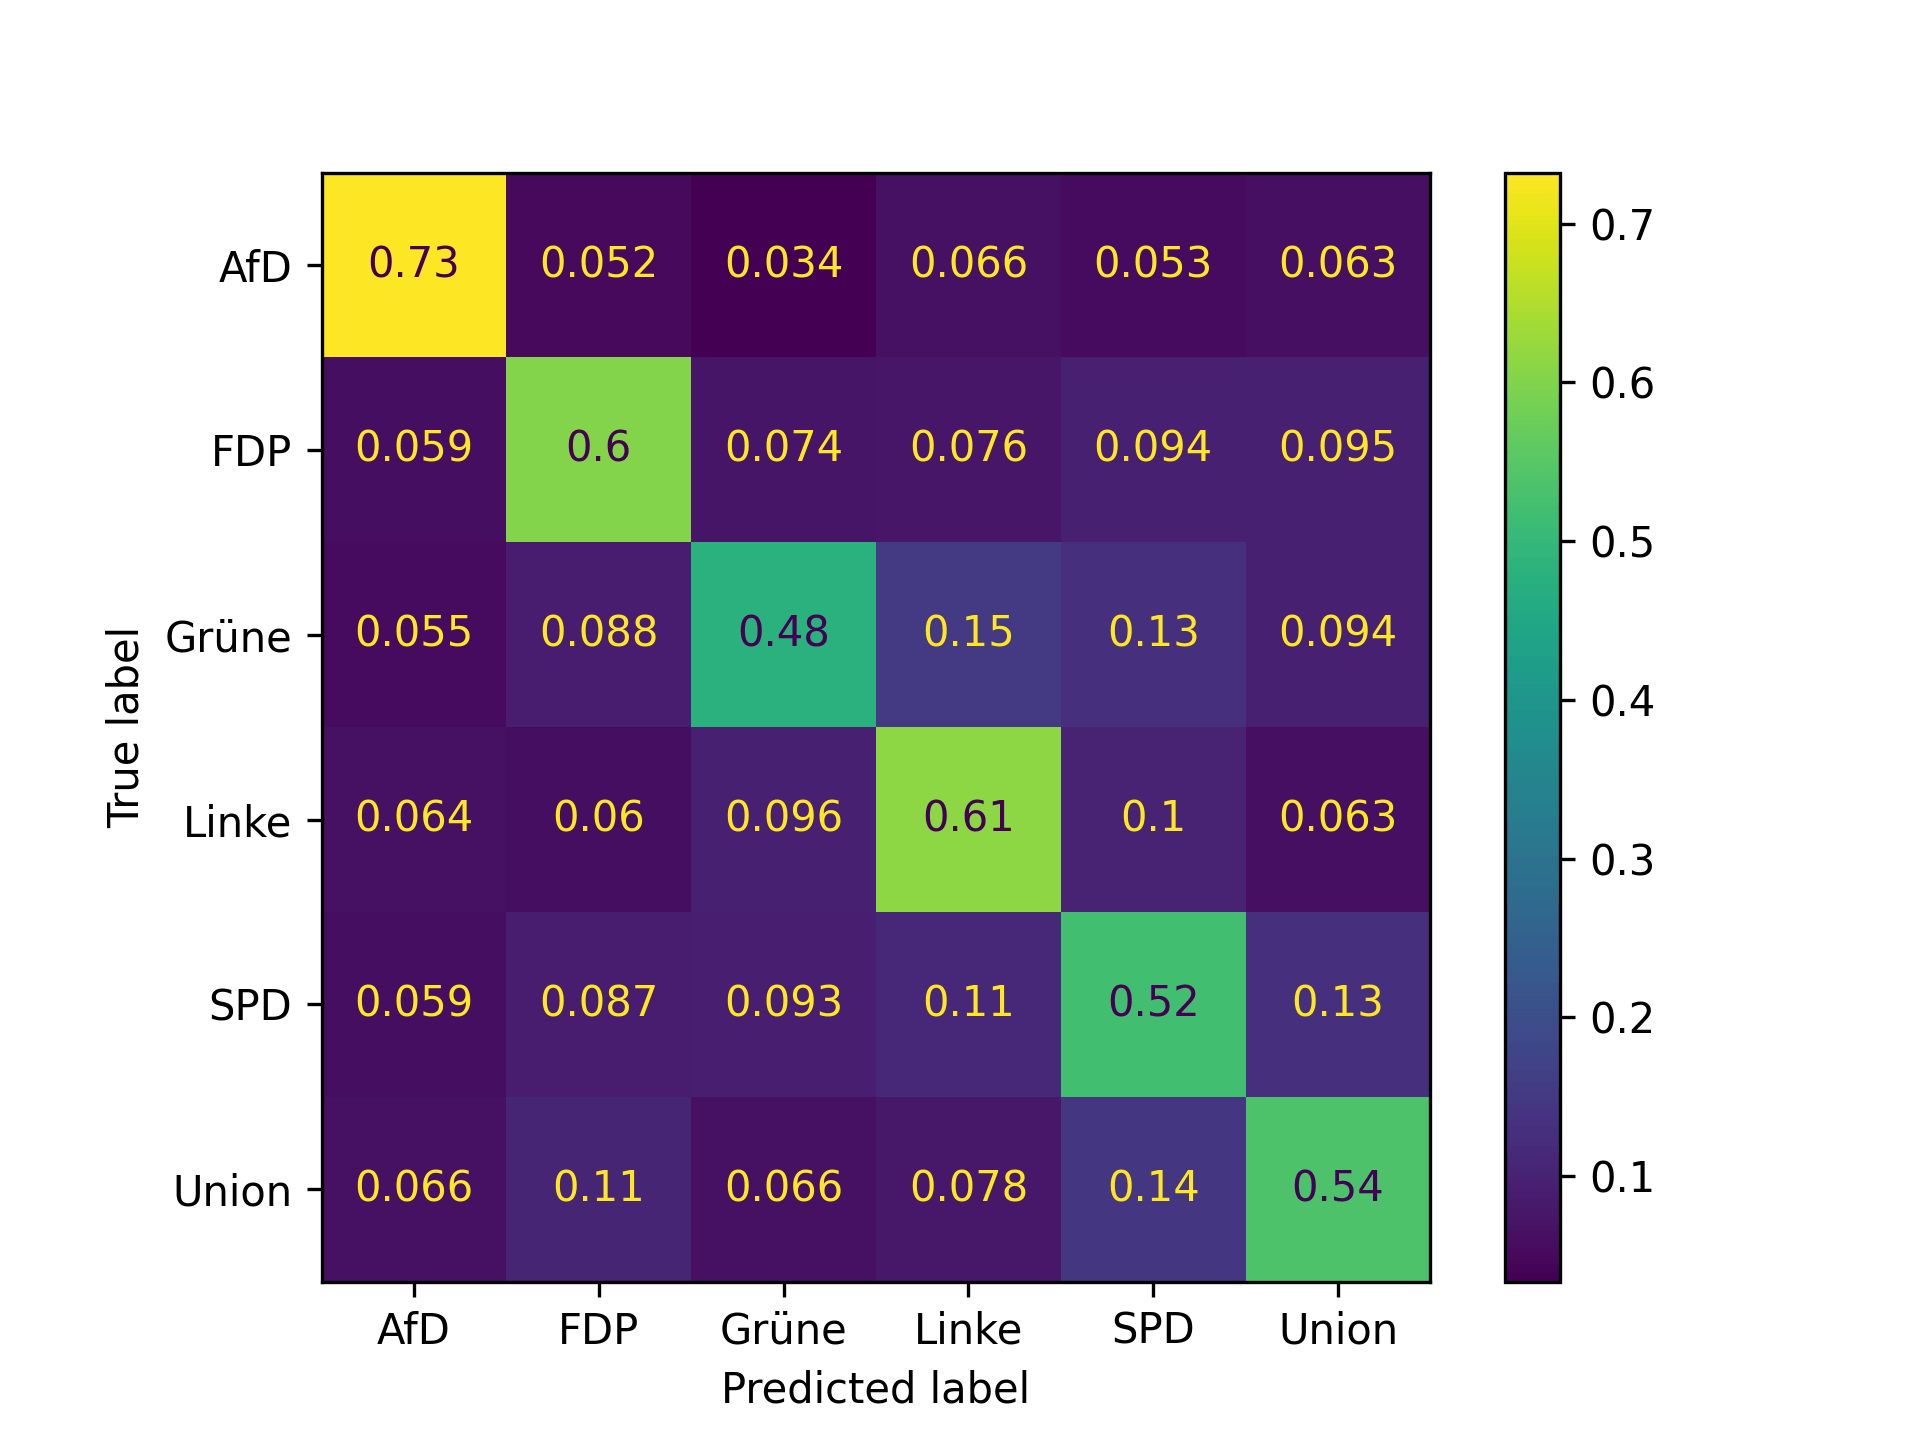
\includegraphics[width=\textwidth]{data/images/modeling/fasttext/under/tweets_confusion_matrix.png}
      \caption{Tweets} \label{sfig:confusionMatrixFastTextTweets}
    \end{subfigure}
    \hfill
    \begin{subfigure}{0.49\textwidth}
      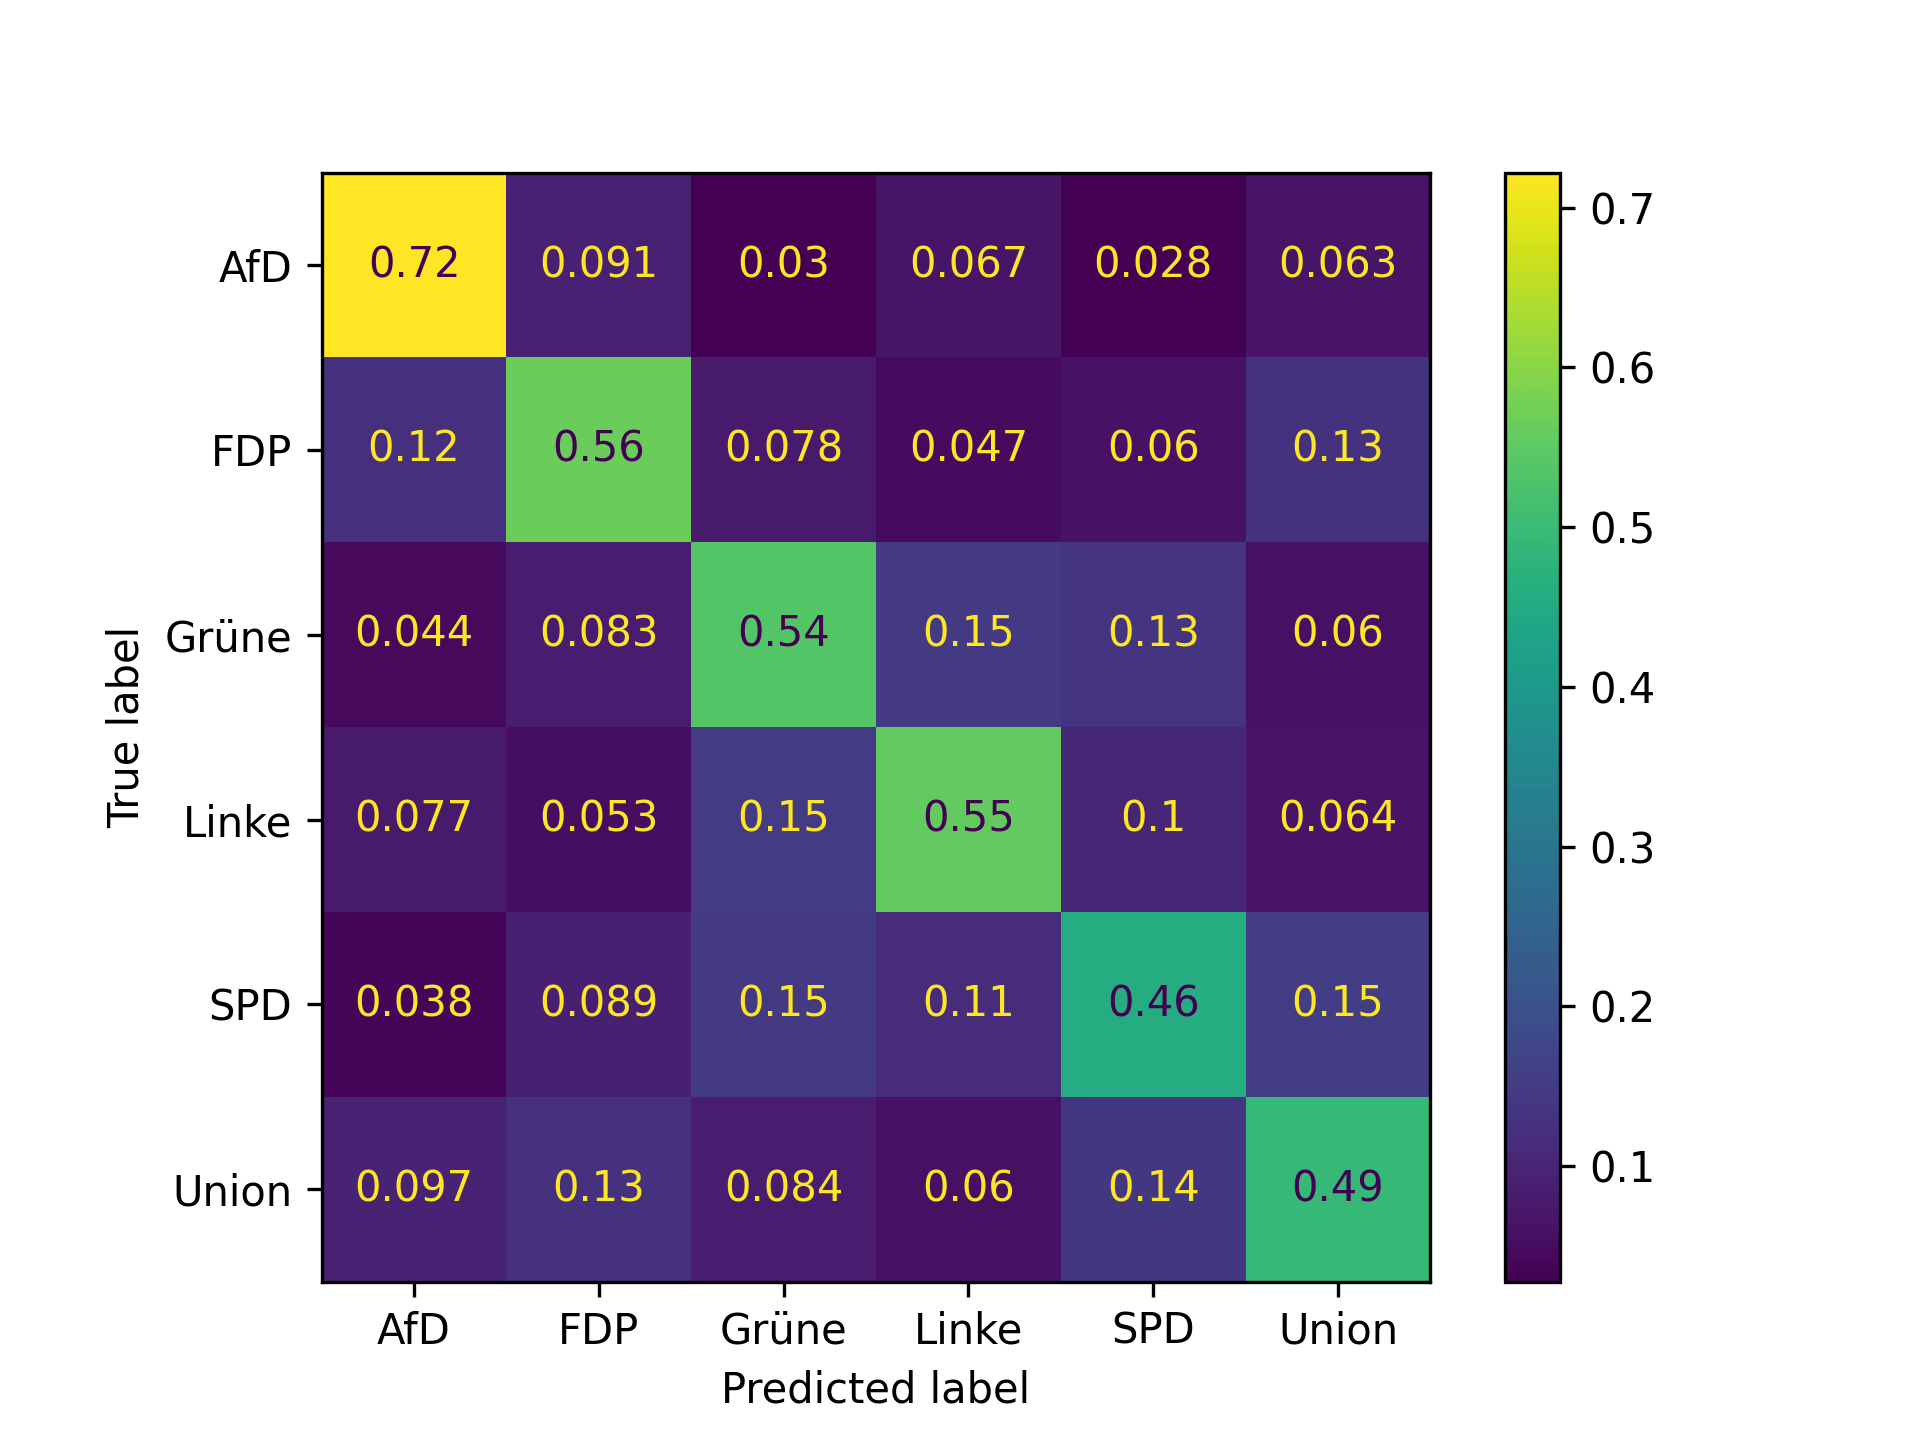
\includegraphics[width=\textwidth]{data/images/modeling/fasttext/under/party_programs_confusion_matrix.png}
      \caption{Wahlprogramme} \label{sfig:confusionMatrixFastTextManifest}
    \end{subfigure}
    \hfill
    \begin{subfigure}{0.49\textwidth}
      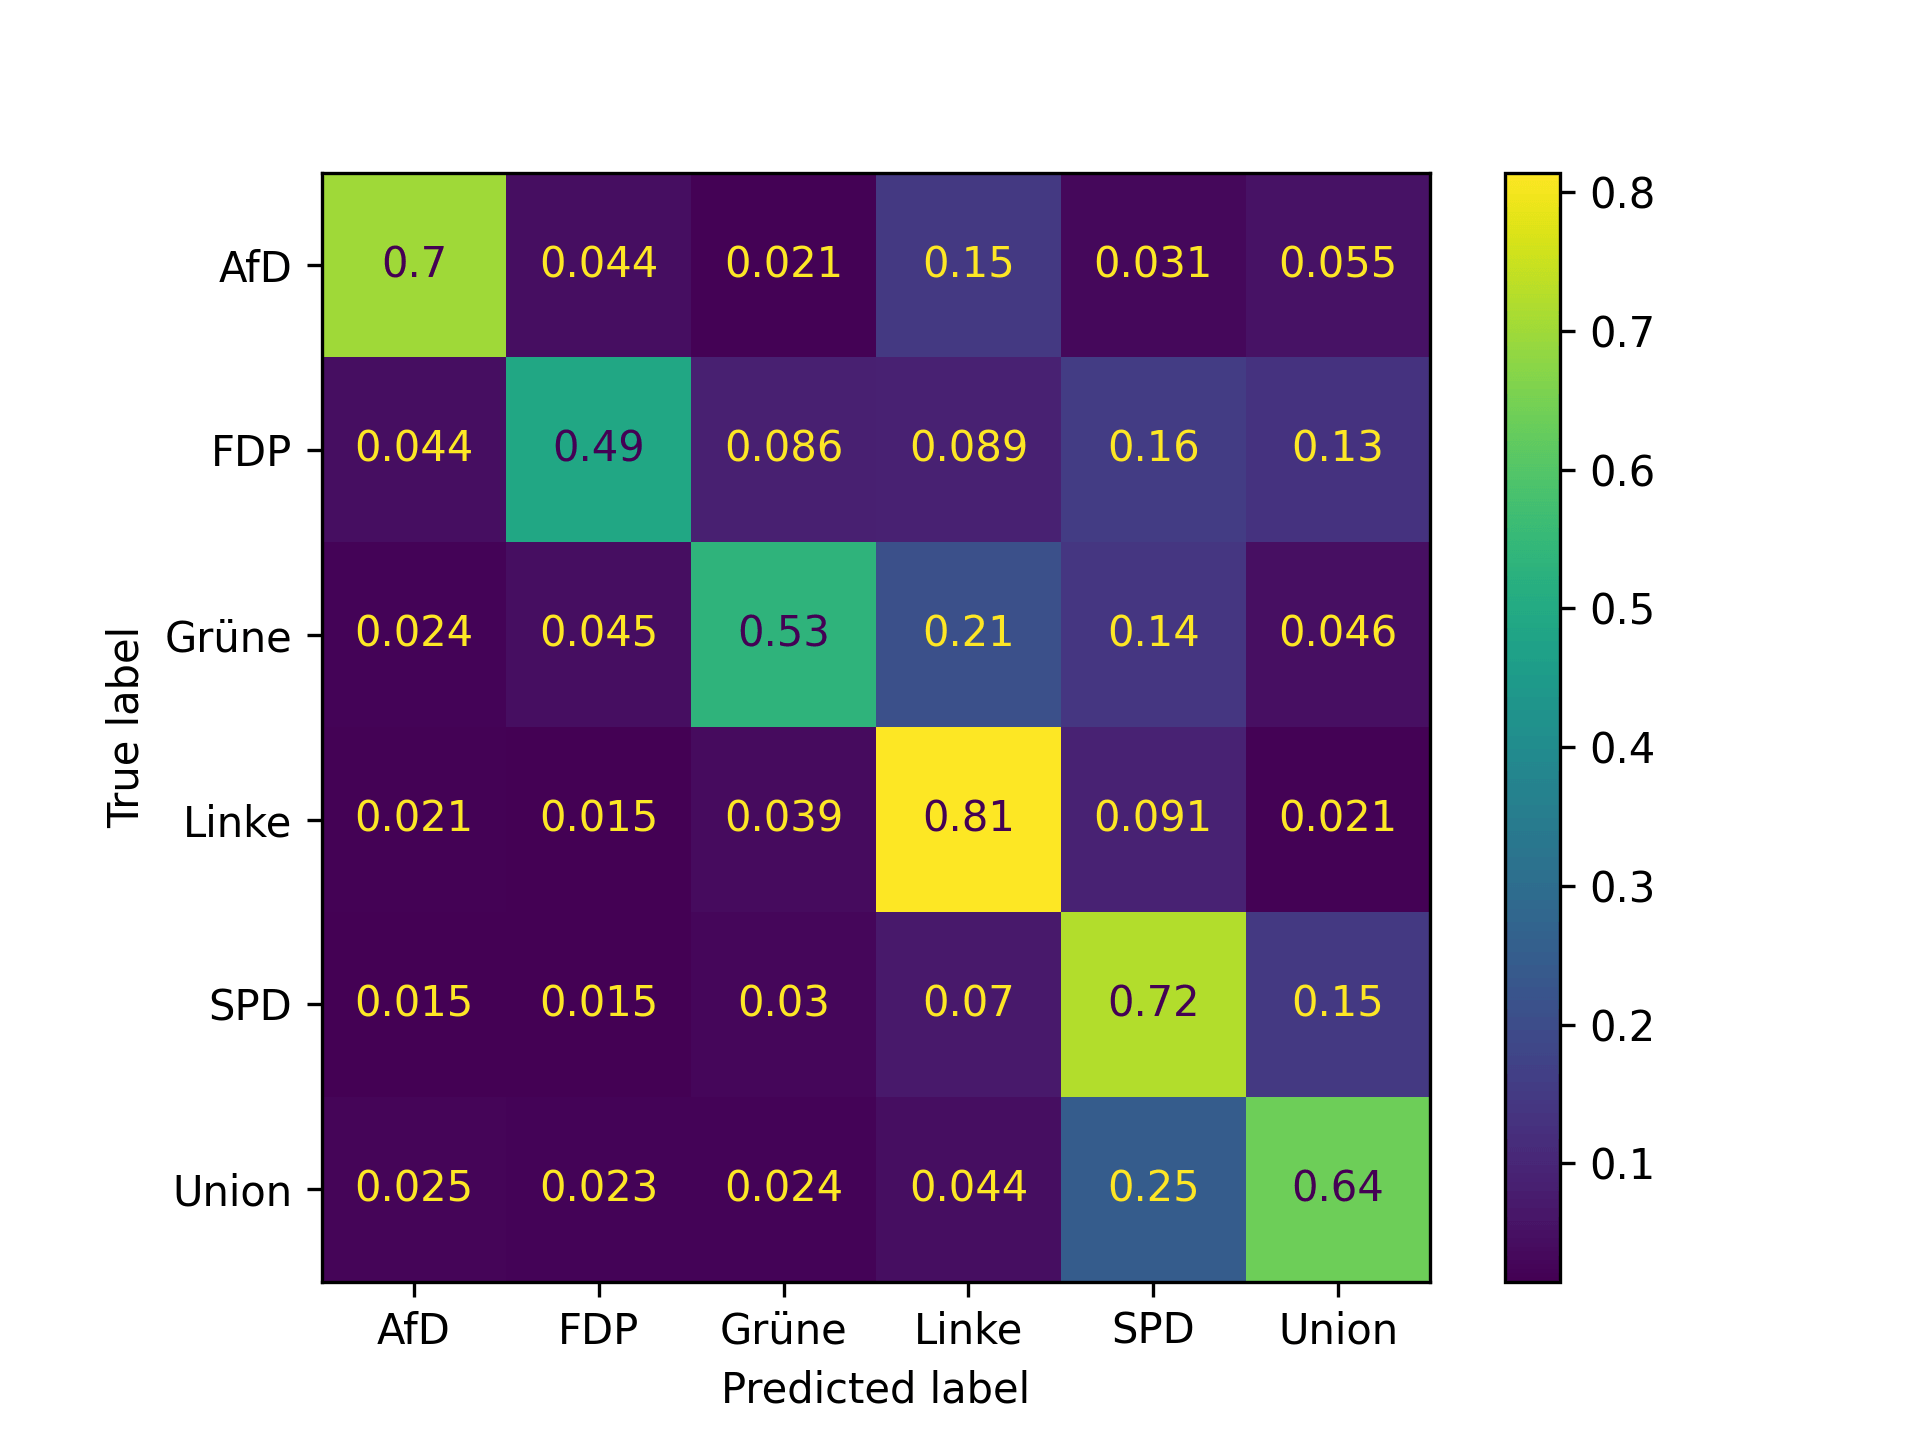
\includegraphics[width=\textwidth]{data/images/modeling/fasttext/under/speeches_confusion_matrix.png}
      \caption{Reden} \label{sfig:confusionMatrixFastTextSpeeches}
    \end{subfigure}
    \hfill
    \begin{subfigure}{0.49\textwidth}
      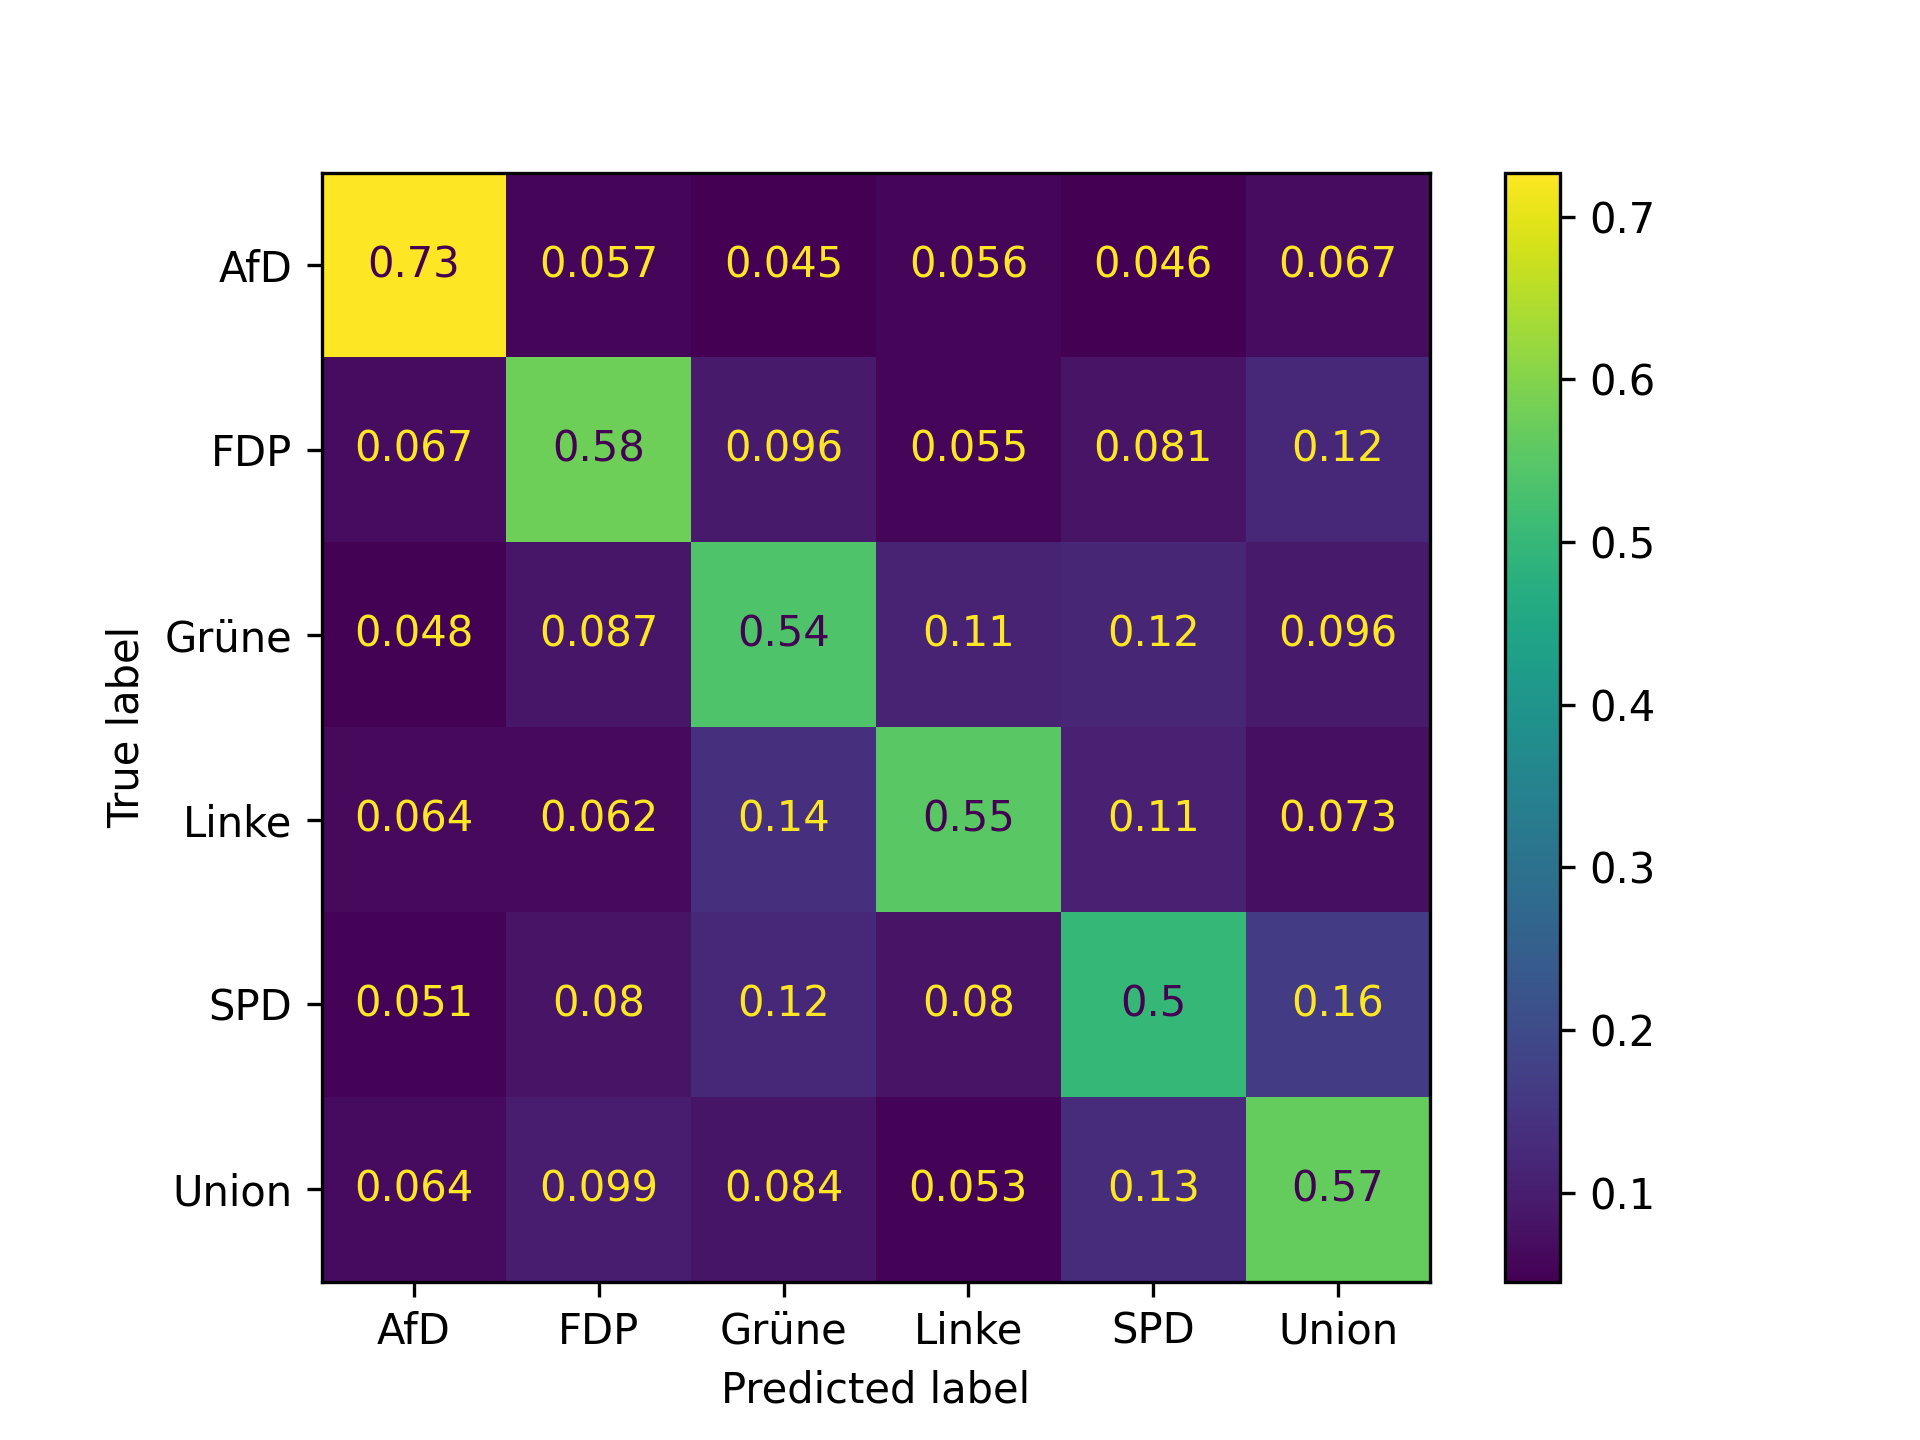
\includegraphics[width=\textwidth]{data/images/modeling/fasttext/under/all_confusion_matrix.png}
      \caption{Kombiniert} \label{sfig:confusionMatrixFastTextAll}
    \end{subfigure}
    \caption{Konfusionsmatrizen für \ft mit Bigrammen (\(n = \num{2}\)) auf ausgeglichenen Datensätzen} \label{fig:confusionMatrixFastText}
\end{figure}

\autoref{sfig:confusionMatrixFastTextTweets} zeigt die Konfusionsmatrix für \ft auf dem Tweet-Datensatz. Die \ac{AfD} erzielt mit \SI{73}{\percent} die höchste Trefferquote. An zweiter Stelle liegen \ac{FDP} und Linke mit jeweils rund \SI{60}{\percent}. Am schlechtesten schneiden die Grünen, die \ac{SPD} und die Union mit einer Trefferquote zwischen \SIrange{48}{54}{\percent} ab. Identisch zu \autoref{sfig:confusionMatrixBaselineTweets} ist festzustellen, dass besonders die linken Parteien (Linke, Grüne und \ac{SPD}) häufig miteinander verwechselt werden. Ähnliche Verwechslungen sind auch zwischen der \ac{FDP} und der Union zu beobachten. Des Weiteren fällt eine hohe Falsch-Negativ-Rate von \SIrange{13}{14}{\percent} zwischen der \ac{SPD} und der Union auf. Im Gegensatz dazu weist die \ac{AfD} konsequent niedrige Verwechselungsraten von maximal \SI{6}{\percent} auf, was darauf hindeutet, dass das Modell diese Partei am zuverlässigsten identifizieren kann.

Bei den Wahlprogrammen in \autoref{sfig:confusionMatrixFastTextManifest} deuten sich erneut ähnliche Muster wie bei \autoref{sfig:confusionMatrixBaselineManifest} an. Zum einen treten die Falsch-Negativ- und Falsch-Positiv-Raten symmetrisch entlang der Richtig-Positiv Achse auf. Zwar lässt sich die \ac{AfD} mit \SI{72}{\percent} ebenfalls am besten klassifizieren, jedoch, im Gegensatz zu \autoref{sfig:confusionMatrixFastTextTweets}, tritt bei der \ac{AfD} und \ac{FDP} eine auffällige Verwechselung von \SIrange{9}{12}{\percent} auf. Identisch zu \autoref{sfig:confusionMatrixFastTextTweets} und \autoref{sfig:confusionMatrixBaselineManifest} weisen Parteien im linken Spektrum eine höher Verwechselungsrate von jeweils \SIrange{10}{15}{\percent} untereinander auf.

\ft weicht auf den Reden stark von den Baseline-Modellen ab. Insbesondere sind Falsch-Negativ-Ergebnisse fast ausschließlich oberhalb der Richtig-Positiv-Achse zu finden. Die Analyse der Richtig-Positiv-Ergebnisse zeigt, dass die Linke mit einer Genauigkeit von \SI{81}{\percent} das beste Ergebnis erzielt, gefolgt von der \ac{AfD} mit einer Genauigkeit von \SI{70}{\percent}. Die \ac{AfD} weißt außerdem eine auffällig hohe Verwechselungsrate von \SI{15}{\percent} mit der Linken auf. Des Weiteren ist auffällig, dass die \ac{FDP} besonders häufig als \ac{SPD} oder Union klassifiziert wird. Ähnliche Verwechslungen treten auch bei den Grünen auf, die weiterhin oft als Linke oder \ac{SPD} klassifiziert werden. Die \ac{SPD} und Union neigen ebenfalls auf den Reden zur Verwechselung. Auffällig ist jedoch, dass Reden der Union zu \SI{25}{\percent} der \ac{SPD} zugeordnet werden. Allgemein fällt auf, dass die \ac{SPD} häufig als Falsch-Positiv klassifiziert wird, was auf einen Bias hin zur \ac{SPD} hindeutet.

Abschließend kann festgestellt werden, dass das Training des Klassifikationsmodells auf dem kombinierten Datensatz ähnliche Muster wie zuvor aufweist, jedoch mit ausgeglicheneren Werten. Die Klassifizierung der \ac{AfD} gelingt erneut mit großem Abstand am besten, was darauf hinweist, dass das Modell charakteristische Merkmale dieser Partei erfolgreich erlernt hat. Bei den restlichen Parteien zeigt sich erneut das Muster, dass das Modell vorwiegend politisch nahestehende Parteien vertauscht. Es fällt auf, dass die \ac{FDP} am ehesten mit der Union verwechselt wird, was darauf hindeutet, dass beide Parteien in bestimmten Kontexten ähnliche Sprachmuster verwenden. Des Weiteren werden die Grünen, die Linke und die \ac{SPD} untereinander häufig verwechselt. Texte der \ac{SPD} werden jedoch hauptsächlich als die der Grünen oder der Union klassifiziert. Wie erwartet zeigt die Union die meisten Verwechselungen mit der \ac{SPD} und der \ac{FDP} auf. Diese könnten auch auf politische Überschneidungen oder Kontroversen in bestimmten Themenbereichen hinweisen, die in den Daten enthalten sind.

\section{Multi-Layer Perceptron}

\sk~bietet durch den \texttt{MLPClassifier} eine einfache Möglichkeit, ein \ac{MLP} für die Klassifikation zu trainieren. Bei einem \ac{MLP} handelt es sich um ein simples neuronales Netzwerk mit einer Eingabeschicht, einer Ausgabeschicht und optionalen Zwischenschichten. Als Eingabedaten wird mittels \ac{BoW} oder \ac{TF-IDF} vektorisierter Text verwendet. Dafür gilt die gleiche Konfiguration wie bereits in \autoref{sec:trainingBaseline} dargelegt sowie die Limitation auf \num{125000} Tweets aus Ressourcengründen.

Eine Hyperparameteroptimierung durch eine Rastersuche liefert als beste Architektur ein Netz mit einer Zwischenschicht bestehend aus \num{100} Neuronen (\(hidden\_layer\_sizes=(\num{100},)\)) sowie der Verwendung der \ac{ReLU}-Aktivierungsfunktion (\(activation=relu\)). Die Lernrate wird initial auf \num{7e-4} gesetzt und nach jeder Iteration graduell verringert (\(learning\_rate=invscaling\)). Das Training in jeder Konfiguration läuft maximal \num{50} Iterationen lang (\(iter\_max=\num{50}\)). Als Eingabetext wird der auf die Wortstämme reduzierte und tokenisierte Text verwendet.

{\footnotesize
\begin{longtblr}[caption={Makro \(F_1\) Score für \acs{MLP}-Modell}, label={tab:overviewScoresMlp}, note{$\dag$}={Aufgrund von beschränkten Rechenressourcen zum Training wird der Datensatz auf \num{125000} zufällig ausgewählte Einträge beschränkt.}, remark{Parameter} = {\(activation=relu\), \(hidden\_layer\_sizes=(\num{100},)\), \(learning\_rate=invscaling\), \(learning\_rate\_init=\num{7e-4}\), \(iter\_max=\num{50}\), \(df\_max = \num{0.2}\), \(ngram\_range = (\num{1}, \num{1})\)}]{hline{1, 3, Z} = {0.75pt}, rowhead = 2, colspec={l*{4}{Q[si={table-format=1.2},c]}}, row{1-2}={guard,font=\bfseries,l}}
     & \SetCell[c=2]{c} BoW & & \SetCell[c=2]{c} TF-IDF & \\
    \cline{2-5}
    Datensatz & Unbalanced & Balanced & Unbalanced & Balanced \\

    Tweets\TblrNote{$\dag$} & \textbf{\num{0.50}} & 0.47 & 0.49 & 0.45 \\
    Wahlpro\-gramme & 0.52 & 0.51 & \textbf{\num{0.54}} & 0.51 \\
    Reden & \textbf{\num{0.66}} & 0.65 & 0.64 & 0.64 \\
\end{longtblr}
}

Das \ac{MLP}-Training dauert mit \SIrange{11}{112}{\minute} deutlich länger als die zuvor dargestellten Ansätze.

In \autoref{tab:overviewScoresMlp} ist der \(F_1\) Score für jede Trainingskombination mit dem \ac{MLP} dargestellt. Für den Tweet- (\num{0.50}) und den Reden-Datensatz (\num{0.66}) kommt die \ac{BoW}-gestützte Variante auf den höchsten Score; bei den Wahlprogrammen jene mit \ac{TF-IDF} (\num{0.54}). Es wird dabei jeweils der unbalancierte Datensatz verwendet. Für jede Repräsentationsform und sowohl auf dem unausgeglichenen als auch auf dem ausgeglichenen Datensätzen erreichen die Wahlprogramme ein besserer Wert als die Tweets und Reden. Das Ergebnis auf dem ausgeglichenen Datensatz liegt stets bis zu \num{0.03} unter dem des unausgeglichenen.

\begin{figure}[H]
\centering
\begin{subfigure}{0.49\textwidth}
    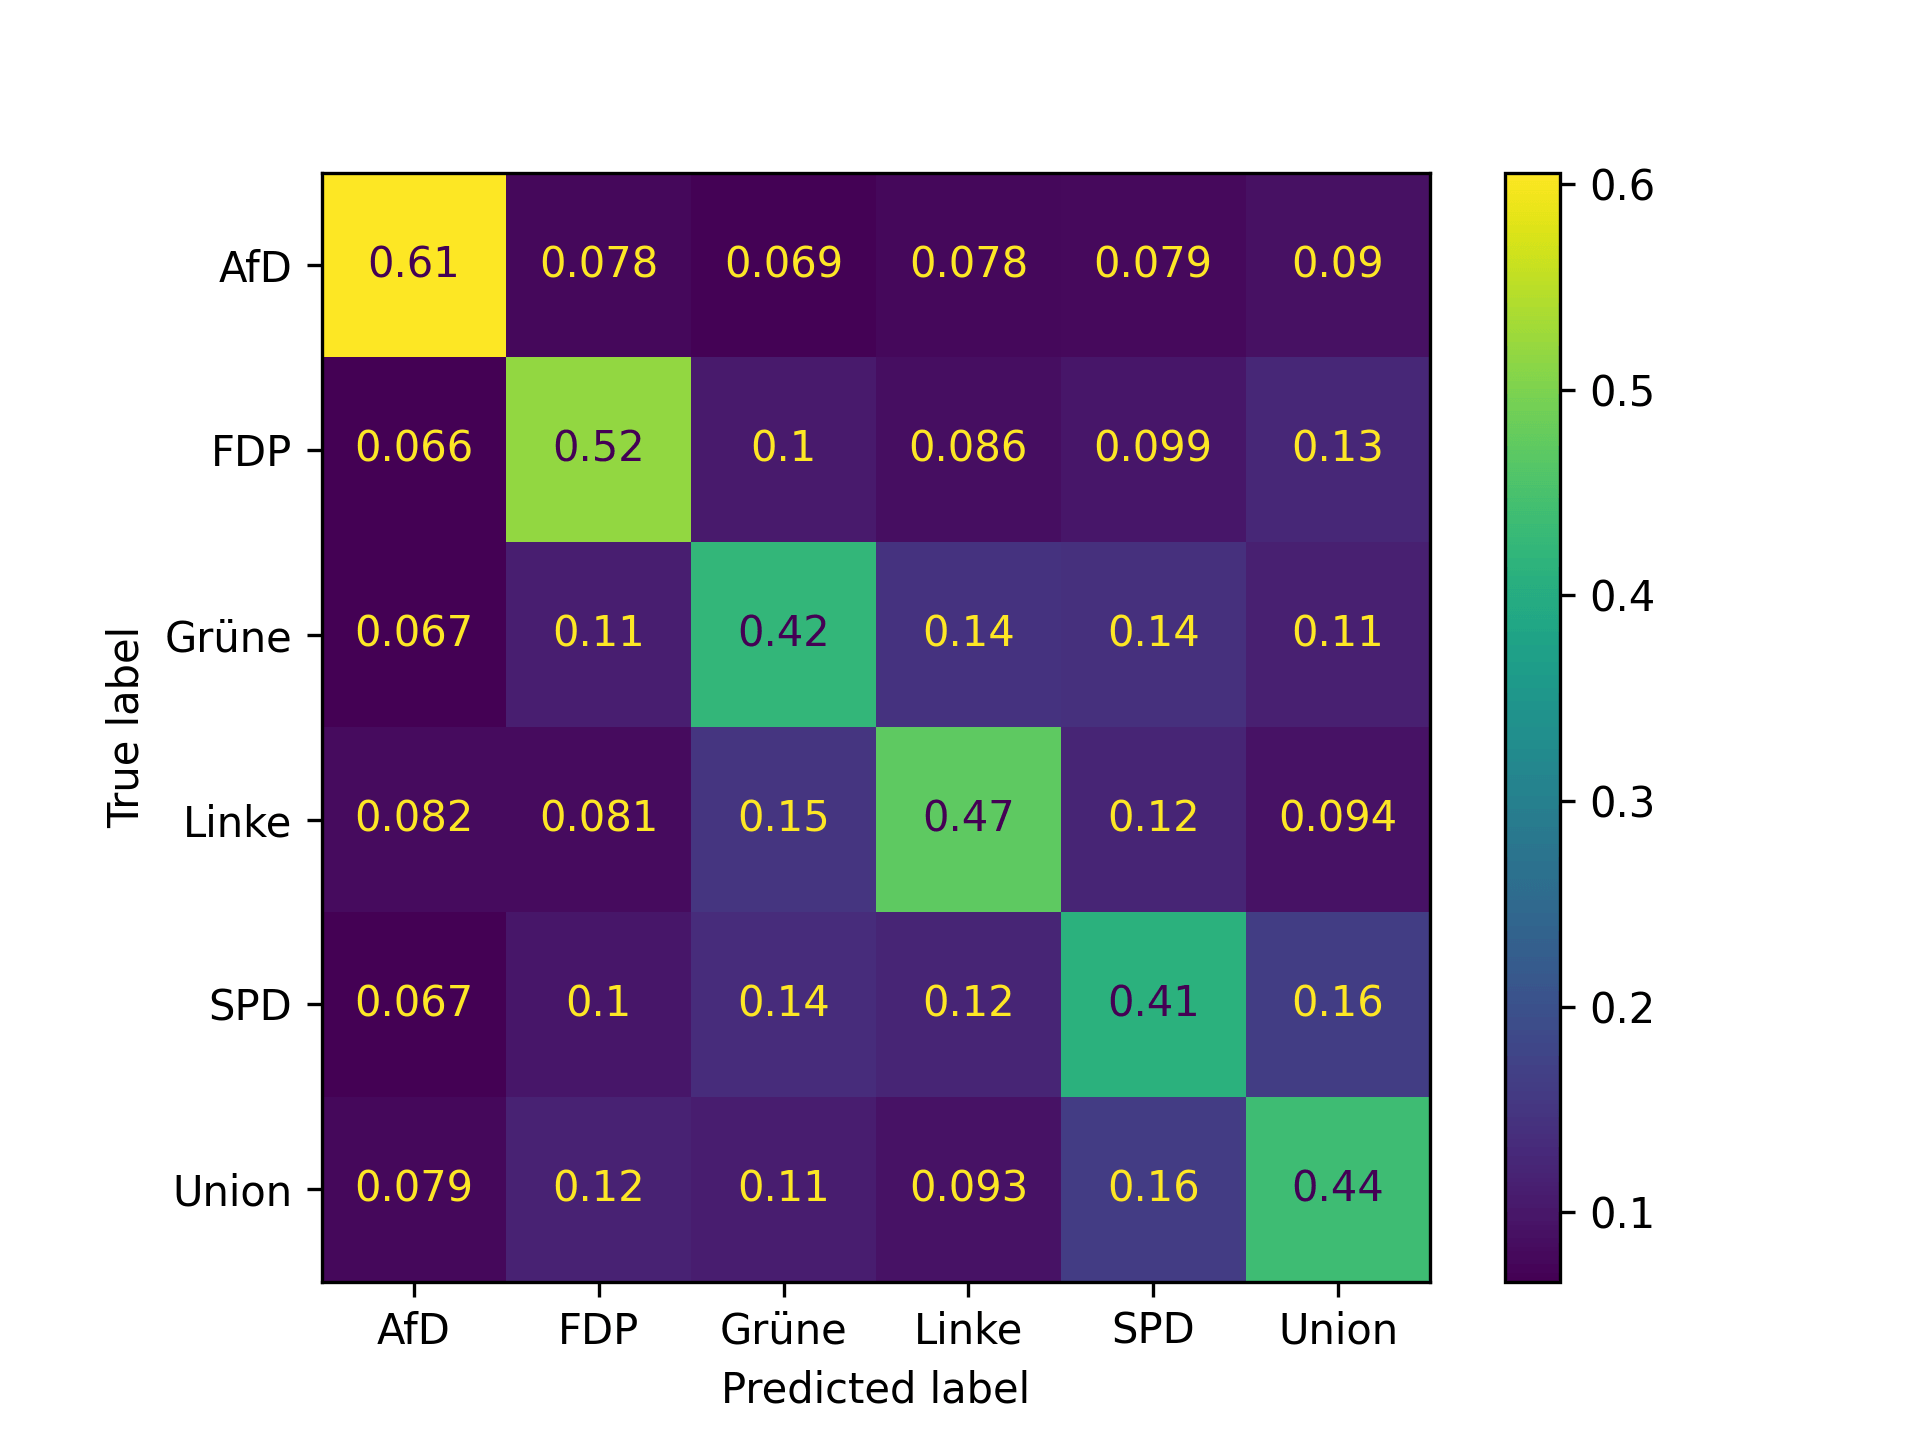
\includegraphics[width=\textwidth]{data/images/modeling/mlp/under/tweets_confusion_matrix.png}
    \caption{Tweets, \ac{BoW}}
    \label{sfig:confusionMatrixMlpTweets}
\end{subfigure}
\hfill
\begin{subfigure}{0.49\textwidth}
    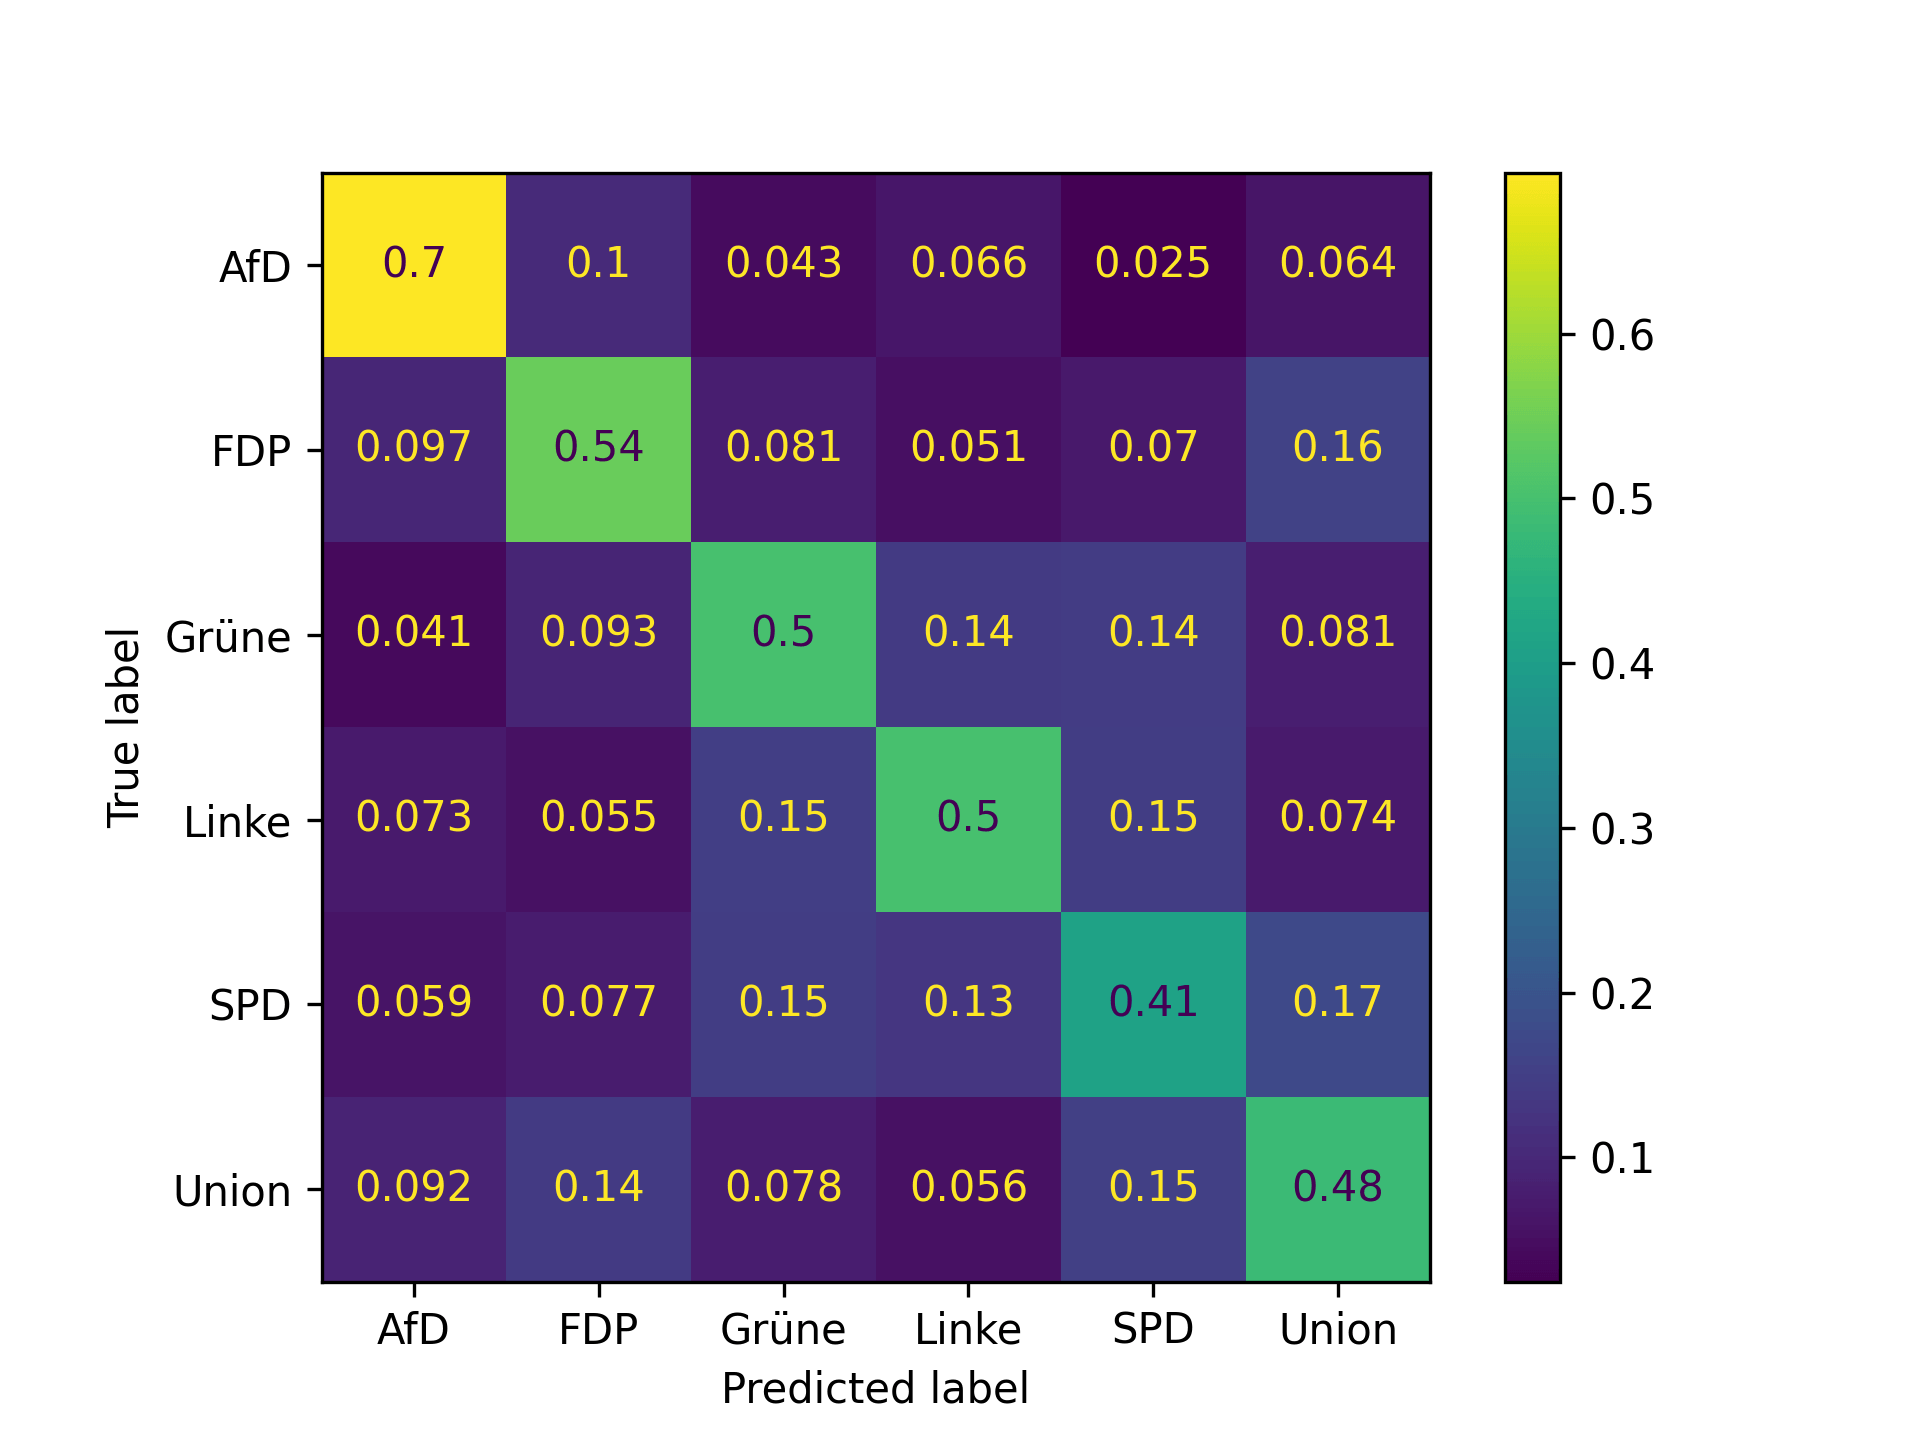
\includegraphics[width=\textwidth]{data/images/modeling/mlp/under/party_programs_confusion_matrix.png}
    \caption{Wahlprogramme, \ac{TF-IDF}}
    \label{sfig:confusionMatrixMlpManifest}
\end{subfigure}
\hfill
\begin{subfigure}{0.49\textwidth}
    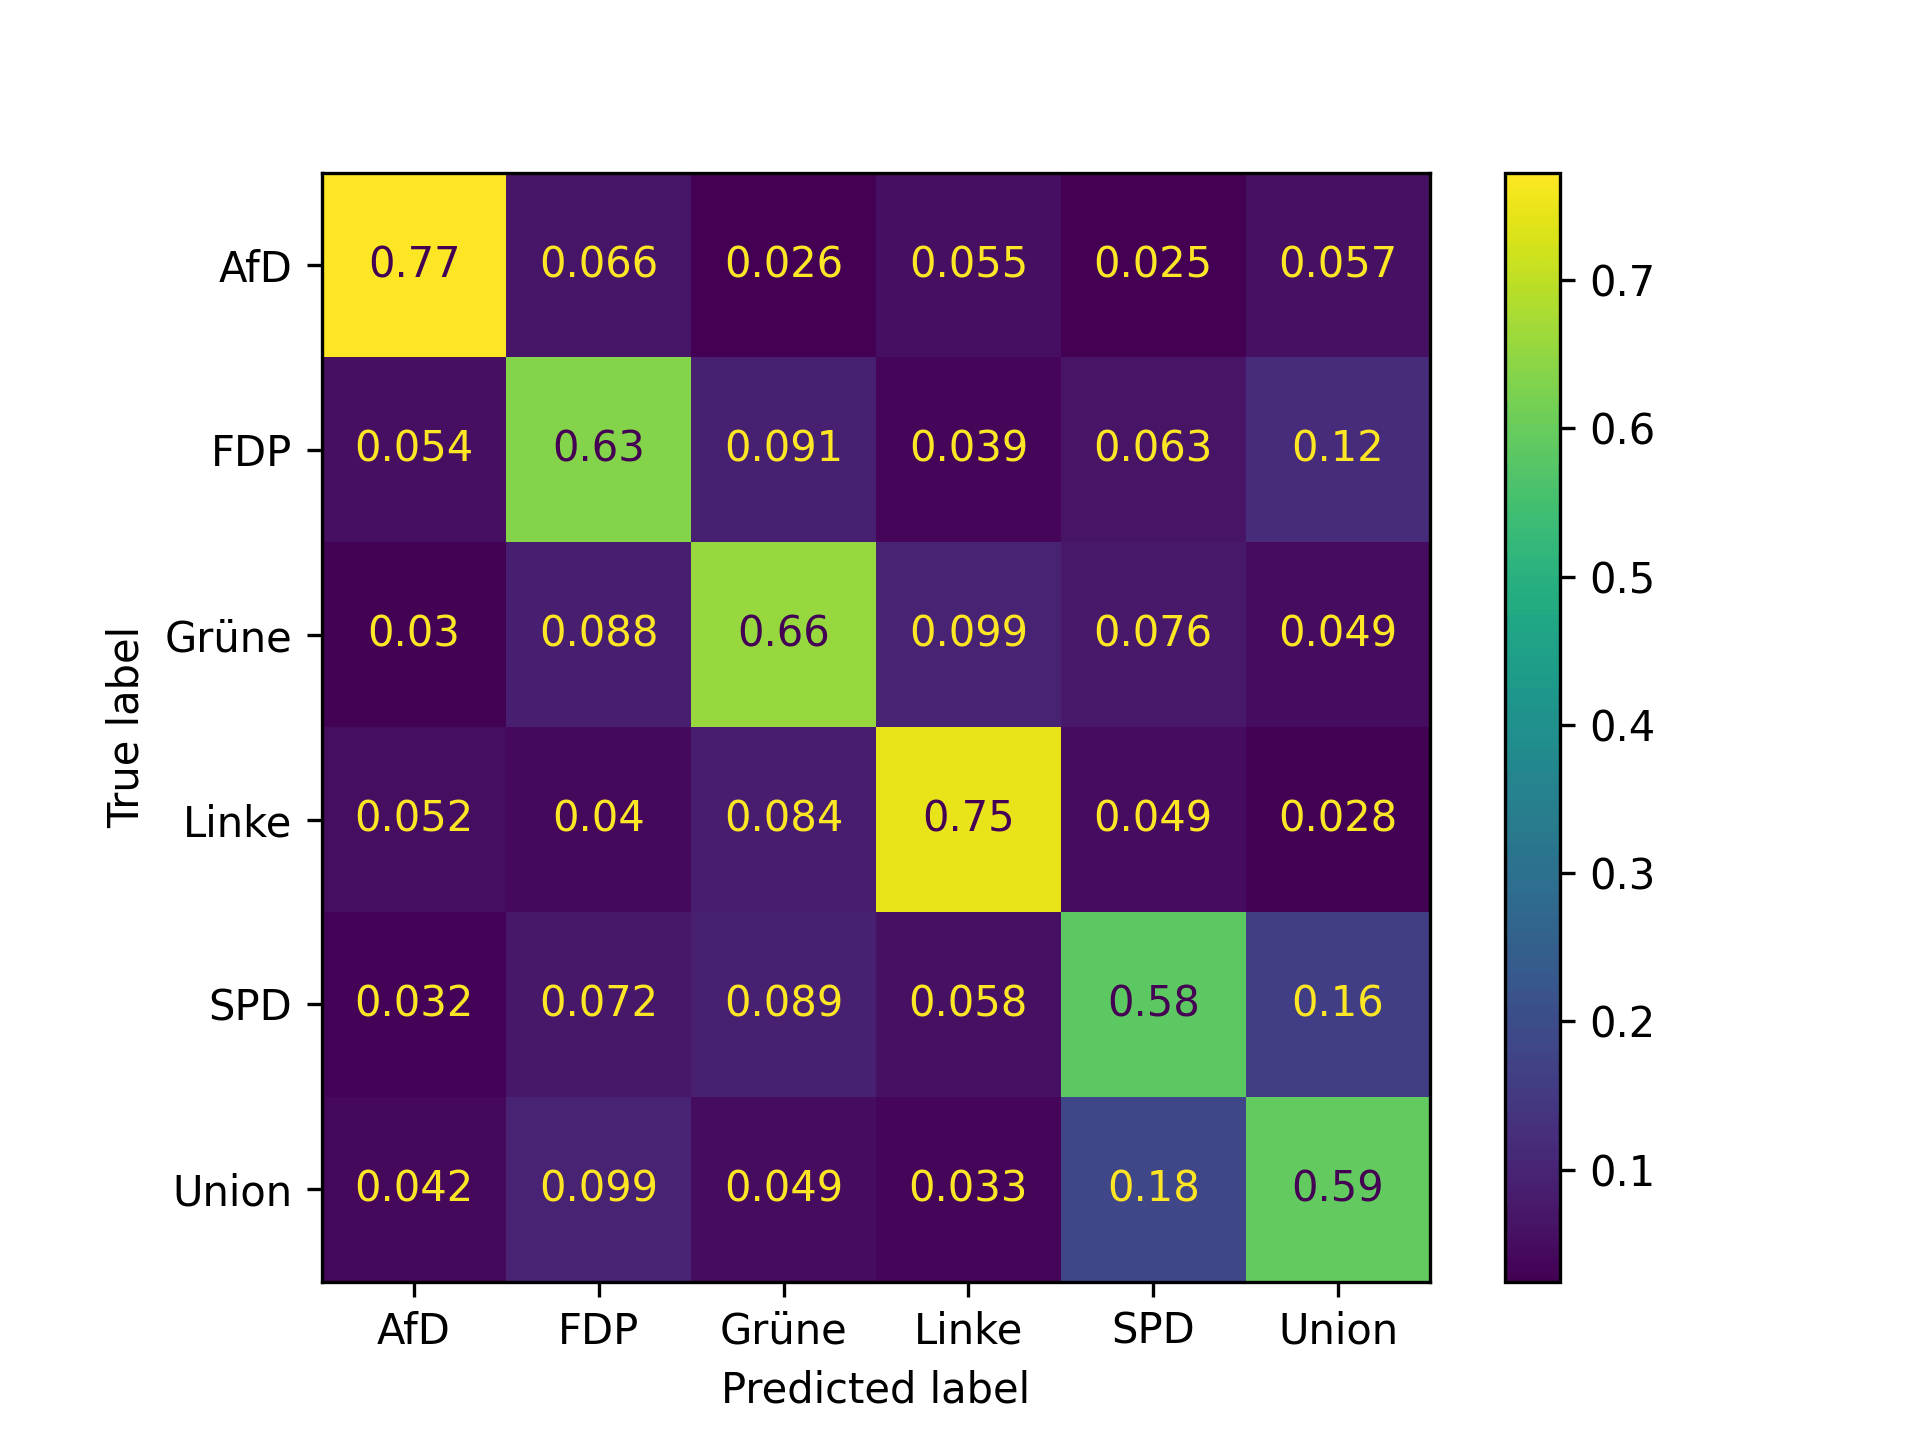
\includegraphics[width=\textwidth]{data/images/modeling/mlp/under/speeches_confusion_matrix.png}
    \caption{Reden, \ac{BoW}}
    \label{sfig:confusionMatrixMlpSpeeches}
\end{subfigure}
\caption{Konfusionsmatrizen für das \acs{MLP}-Modell auf ausgeglichenen Datensätzen} \label{fig:confusionMatrixMlp}
\end{figure}

\autoref{sfig:confusionMatrixMlpTweets} zeigt die Konfusionsmatrix des \ac{MLP}-Modells für den Tweet-Datensatz. Die mit Abstand beste Richtig-Positiv-Rate erreicht die \ac{AfD} (\SI{61}{\percent}). Die Falsch-Negativen-Anteile der \ac{AfD}-Tweets sind relativ gleich auf die anderen Parteien verteilt. Das zweitbeste Ergebnis erreicht die \ac{FDP}, deren Tweets zu \SI{54}{\percent} korrekt erkannt und hauptsächlich nur mit der Union verwechselt werden. Bei den Grünen ergeben sich die höchsten Falsch-Negativ-Werte bei der Linken und \ac{SPD}, wobei auch \ac{FDP} und Union mit je \SI{11}{\percent} häufig vertreten sind. Auffällig ist, dass Grüne und \ac{SPD} insgesamt oft -- bei allen Parteien außer der \ac{AfD} -- falsch-positiv klassifiziert werden. Die Parteien mit den meisten Falsch-Negativ-Werten sind bei der \ac{SPD} Union, Grüne und Linke und bei der Union \ac{SPD} und \ac{FDP}. Die Konfusionsmatrix der Tweets ist annähernd symmetrisch entlang der Richtig-Positiv-Achse.

Bei den Wahlprogrammen in \autoref{sfig:confusionMatrixMlpManifest} ergibt sich ein fast identisches Bild. Dabei bestehen dennoch wesentliche Unterschiede: Einerseits sind die Falsch-Negativ-Werte für \ac{AfD}-Wahlprogramm-Abschnitte ungleicher verteilt, mit einem Schwerpunkt bei der \ac{FDP} mit \SI{10}{\percent}. Dabei ist die Richtig-Positiv-Rate der \ac{AfD} mit \SI{70}{\percent} signifikant höher als bei den Tweets. Zudem ist die gegenseitige Verwechslung zwischen \ac{FDP} und Union mit \SI{16}{\percent} beziehungsweise \SI{14}{\percent} stärker ausgeprägt. Auch besteht mit \SI{15}{\percent} eine auffällig höhere Falsch-Negativ-Rate bezüglich der \ac{SPD} bei den Einträgen der Linken.

Die Konfusionsmatrix der Reden in \autoref{sfig:confusionMatrixMlpSpeeches} enthält, ähnlich wie in der analogen \autoref{sfig:confusionMatrixBaselineSpeeches} für die Baseline-Modelle dargestellt, vor allem auffällig hohe Falsch-Negativ-Werte zwischen den Parteien der Großen Koalition, \ac{SPD} und Union.

\section{Convolutional Neural Network}

Als weiteren Ansatz, der auf neuronalen Netzen basiert, wird im Folgenden ein \ac{CNN}-Modell für die Textklassifikation genutzt. \autoref{fig:cnnArchitecture} stellt die Architektur des zum Training genutzten \ac{CNN} dar.

\begin{figure}[H]
  \centering
  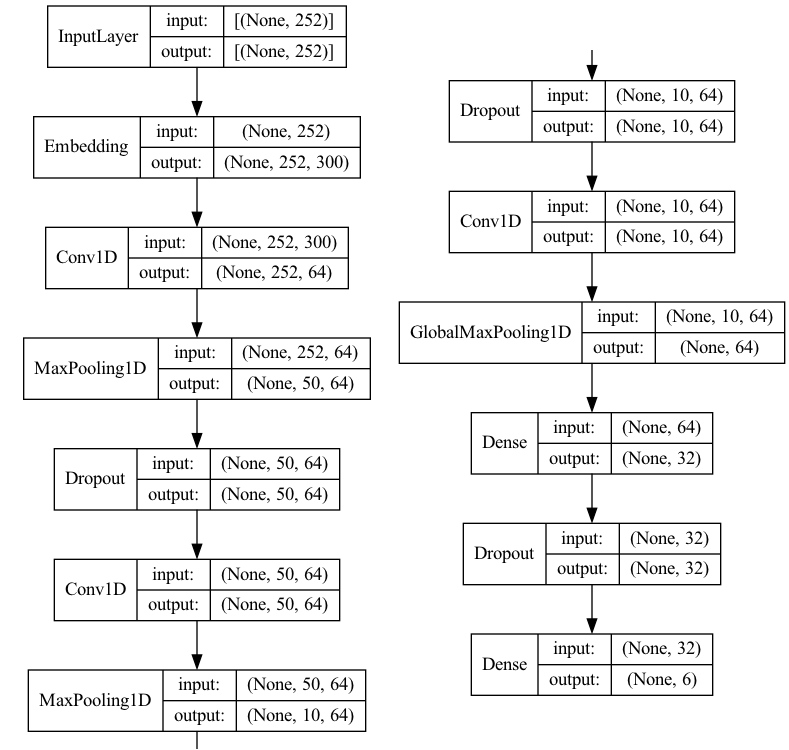
\includegraphics[width=0.6\textwidth]{data/images/cnn.png}
  \caption{Übersicht über die \acs{CNN}-Archtitektur} \label{fig:cnnArchitecture}
\end{figure}

In die Eingabeschicht wird der Text übergeben und transformiert. Die maximale Anzahl an Tokens beläuft sich hierbei auf \num{252}. Diese Obergrenze passt dich dynamisch an den Trainingsdatensatz an, indem das \SI{99}{\percent} Perzentil der Tokenzahl der Einträge gewählt wird. Dadurch wird der überwiegende Teil der Texte vollständig verarbeitet, aber vermieden, dass Ausreißer für eine große Eingabelänge aller Daten sorgen. Jeder Text wird, wenn er kürzer als die maximale Tokenzahl ist, bis zu dieser aufgefüllt. Der übrige Teil wird verworfen. Anschließend wird der tokenisierte Text in die Embedding-Schicht übergeben, in der die Tokens mit den zugehörigen Wortvektoren ausgetauscht werden. In diesem Fall handelt es sich um deutsche \ac{GloVe} Worteinbettungen\footnote{\href{https://www.deepset.ai/german-word-embeddings}{https://www.deepset.ai/german-word-embeddings}} mit der Dimension \num{300}. Es folgt zweimal die Kombination aus einer \textit{Convolution}- (mit \num{64} Filtern), \textit{MaxPooling}- und \textit{Drop-out}-Schicht (mit einer Rate von \SI{30}{\percent}). Im Anschluss ist eine erneute \textit{Convolution}- gefolgt von einer \textit{GlobalMaxPooling}-Schicht vorgesehen. Mittels der globalen MaxPooling Schicht werden die Daten auf eine Dimension reduziert. Zum Schluss beinhaltet das \ac{CNN} eine \textit{Dense}- (mit 32 Neuronen) und \textit{Drop-out}-Schicht (ebenfalls mit einer Rate von \SI{30}{\percent}), bevor die Ausgabeschicht mit sechs Neuronen -- die Anzahl an Klassen (Parteien) -- das Ende des \ac{CNN} bildet. Die Softmax-Aktivierungsfunktion in der Ausgabeschicht stellt schlussendlich sicher, dass die Summe der Ausgabewahrscheinlichkeiten aller Parteien \SI{100}{\percent} beträgt.

{\footnotesize
\begin{longtblr}[caption={Makro \(F_1\) Score für \acs{CNN}-Modell}, label={tab:overviewScoresCNN}, remark{Parameter} = {\(E = \num{20}\), \(LR = \num{7.5e-4}\), \(B = \num{64}\)}]{width=\textwidth, hline{1-2, Y-Z} = {0.75pt}, colspec={l*{2}{Q[si={table-format=1.2},c]}}, row{1}={guard,font=\bfseries,l}}
    Datensatz & Unbalanced & Balanced \\ 

    Tweets & \textbf{\num{0.46}} & 0.44 \\*
    Wahlprogramme & \textbf{\num{0.48}} & 0.44 \\*
    Reden & \textbf{\num{0.58}} & 0.53 \\*
    
    Kombiniert & \textbf{\num{0.48}} & 0.47 \\ 
\end{longtblr}
}

Die Trainingsdauer des \ac{CNN} beträgt \SIrange{2}{19}{\minute}. Das Modell lässt sich somit deutlich schneller als das \ac{MLP}, jedoch langsamer als die Baseline-Modelle und \ft, trainieren. Anders als bei den vorherigen Modellen werden die lediglich bereinigten, aber nicht tokenisierten Daten verwendet.

\autoref{tab:overviewScoresCNN} stellt die Trainingsergebnisse des \ac{CNN} auf unausgeglichenen und ausgeglichenen Daten dar. Für jeden Datensatz liefert der unausgeglichene Datensatz einen höheren \(F_1\) Score als der ausgeglichenen. Die Tweets zeigen mit \num{0.46} den niedrigsten Score für unausgeglichene Daten auf (ausgeglichen: \num{0.44}), gefolgt von den Wahlprogrammen mit \num{0.48} (ausgeglichen: \num{0.44}). Die mit Abstand beste Performance lässt sich -- wie auch bei den vorangegangenen Modellen -- durch den Reden-Datensatz erzielen (\num{0.58}; ausgeglichen: \num{0.53}). Das Training auf dem kombinierten Datensatz liefert einen \(F_1\) Wert von \num{0.48} auf dem unbalancierten und \num{0.47} auf dem balancierten Datensatz.

\begin{figure}[H]
    \centering
    \begin{subfigure}{0.49\textwidth}
        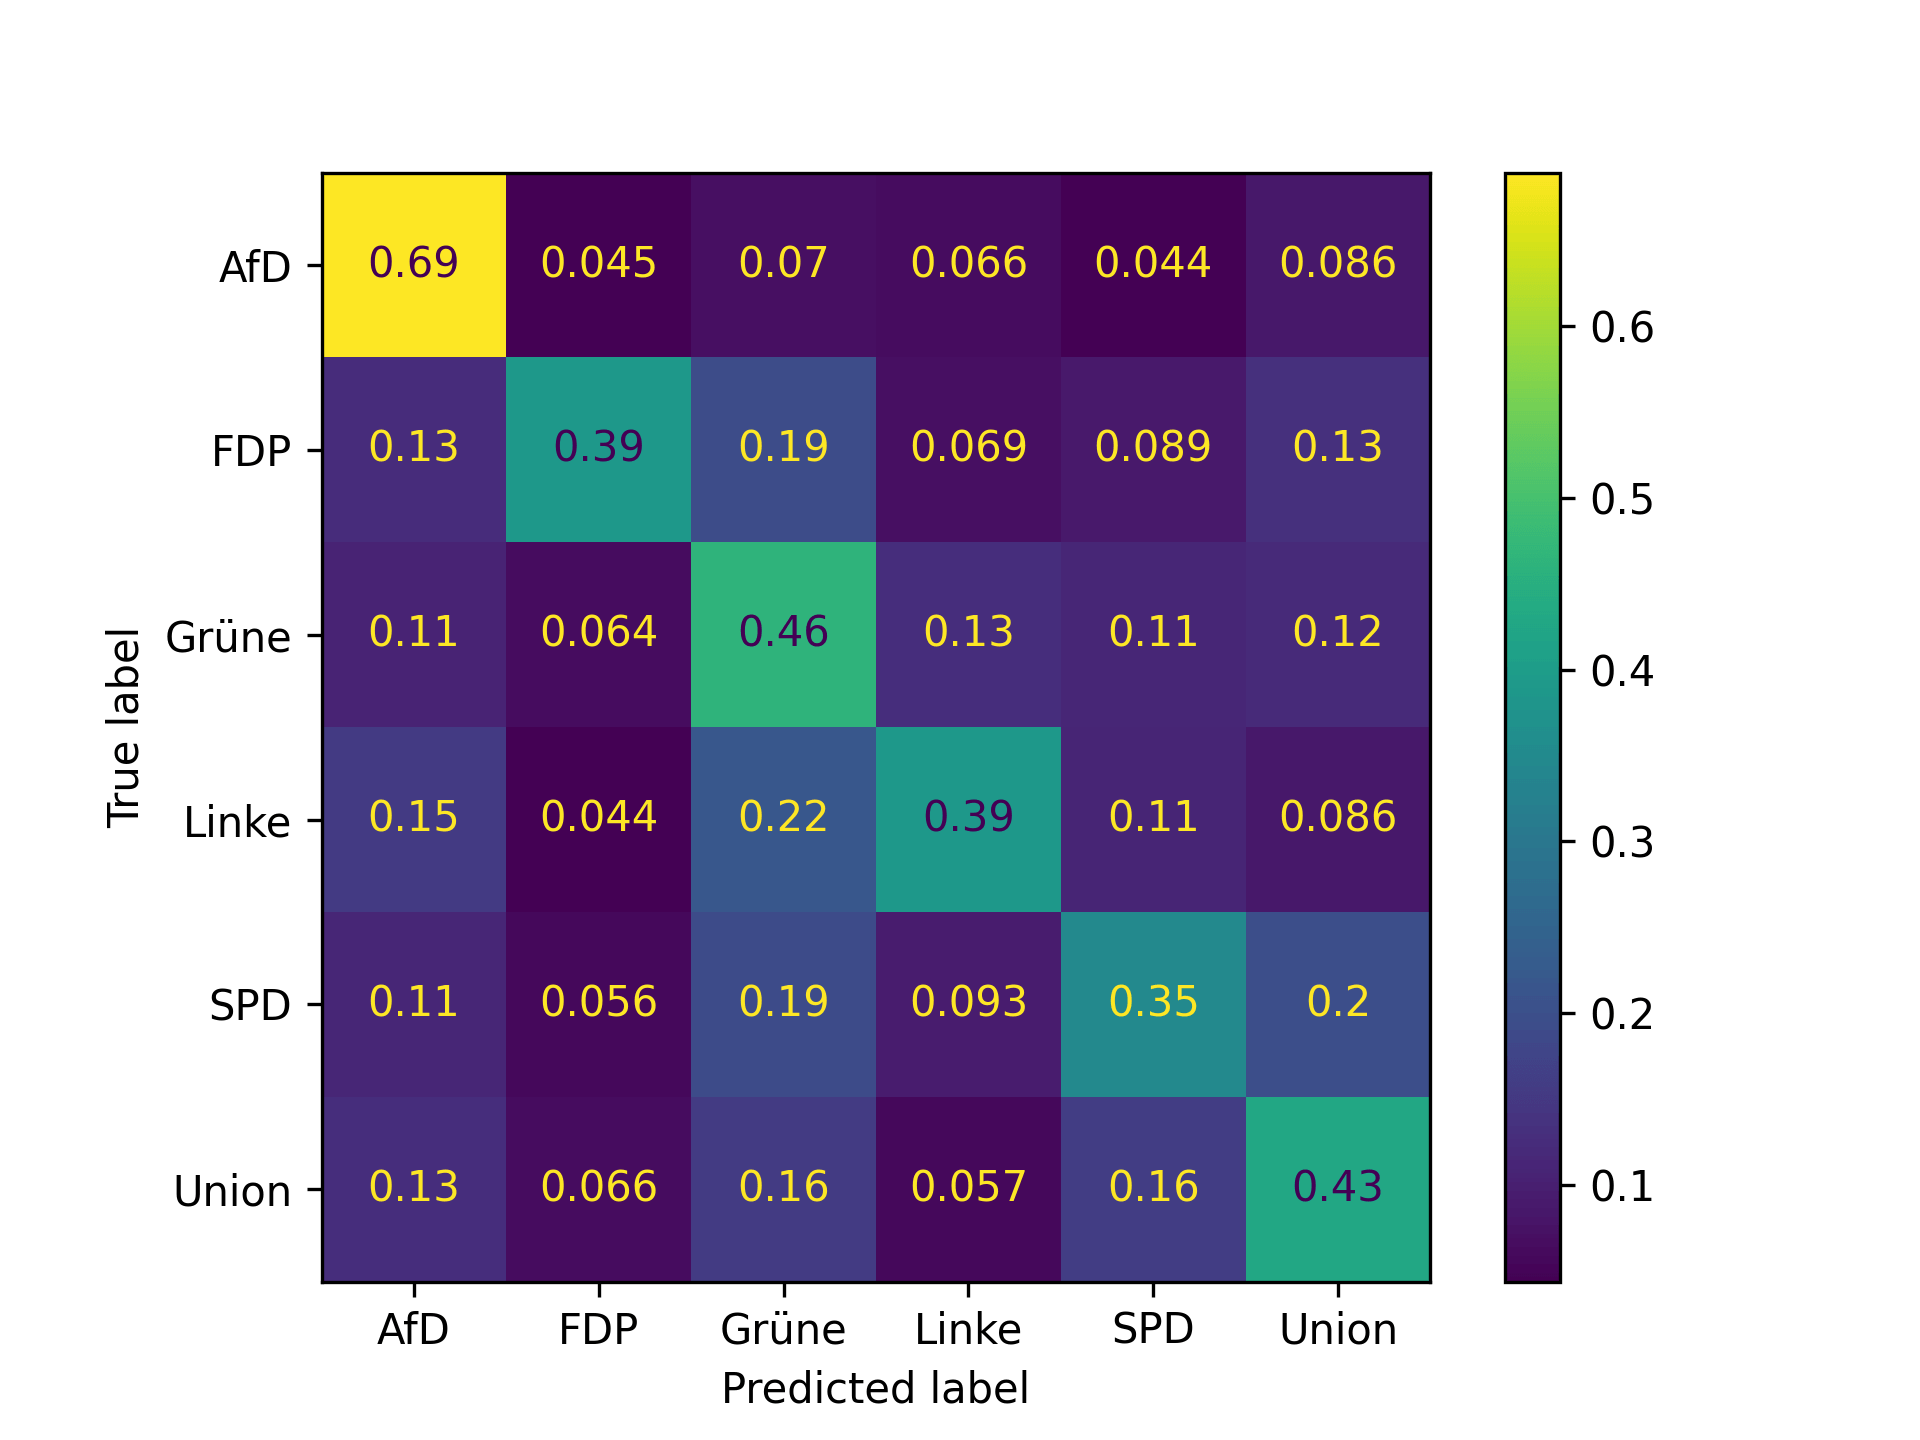
\includegraphics[width=\textwidth]{data/images/modeling/cnn/under/tweets_confusion_matrix.png}
        \caption{Tweets}
        \label{sfig:confusionMatrixCnnTweets}
    \end{subfigure}
    \hfill
    \begin{subfigure}{0.49\textwidth}
        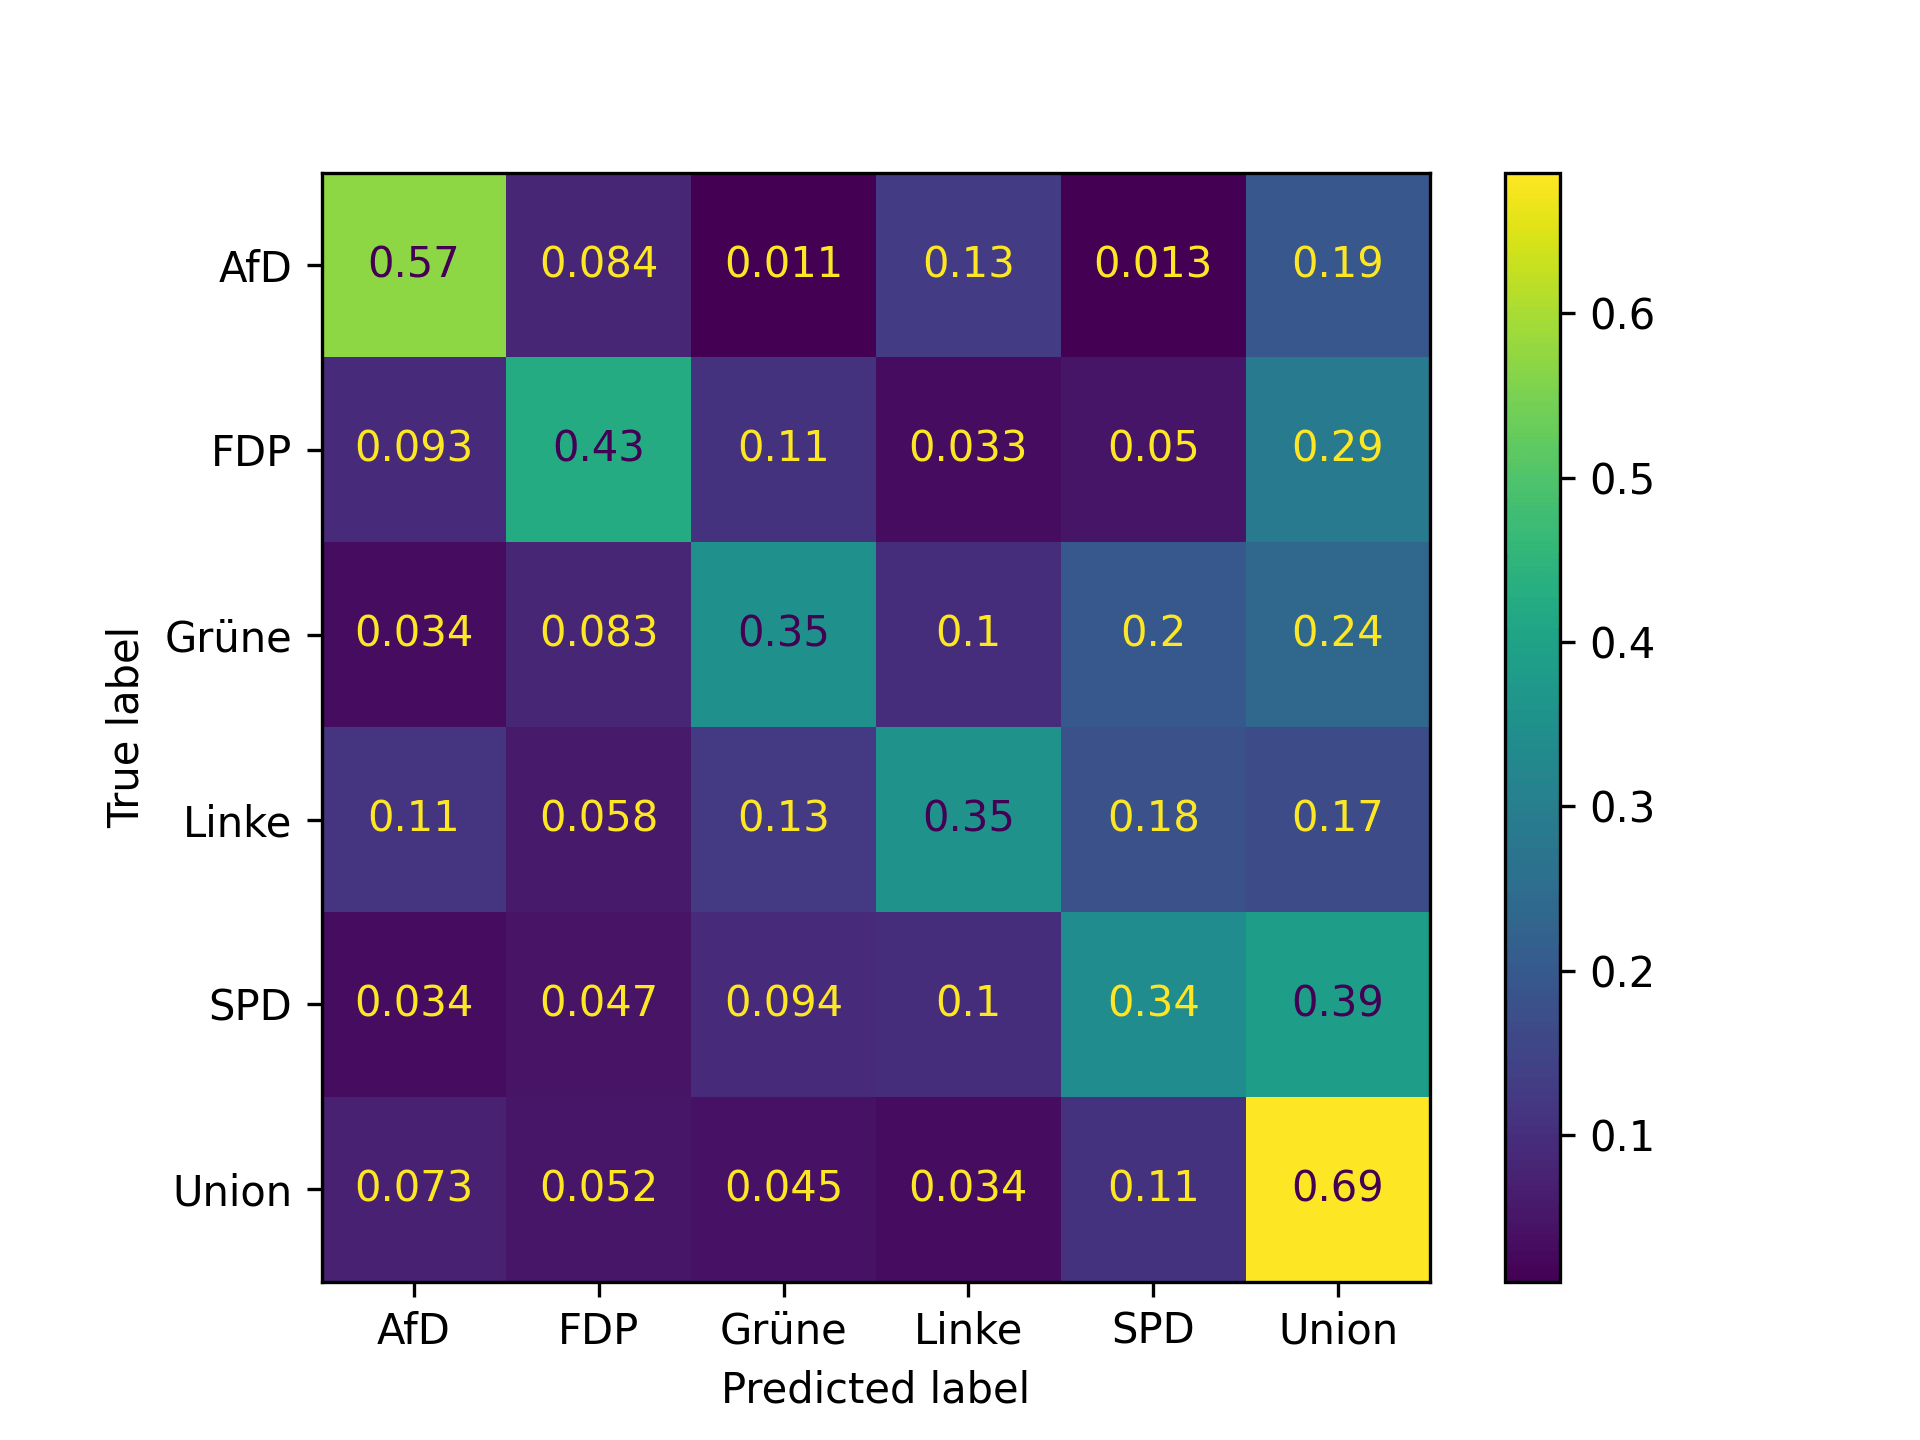
\includegraphics[width=\textwidth]{data/images/modeling/cnn/under/party_programs_confusion_matrix.png}
        \caption{Wahlprogramme}
        \label{sfig:confusionMatrixCnnManifest}
    \end{subfigure}
    \hfill
    \begin{subfigure}{0.49\textwidth}
        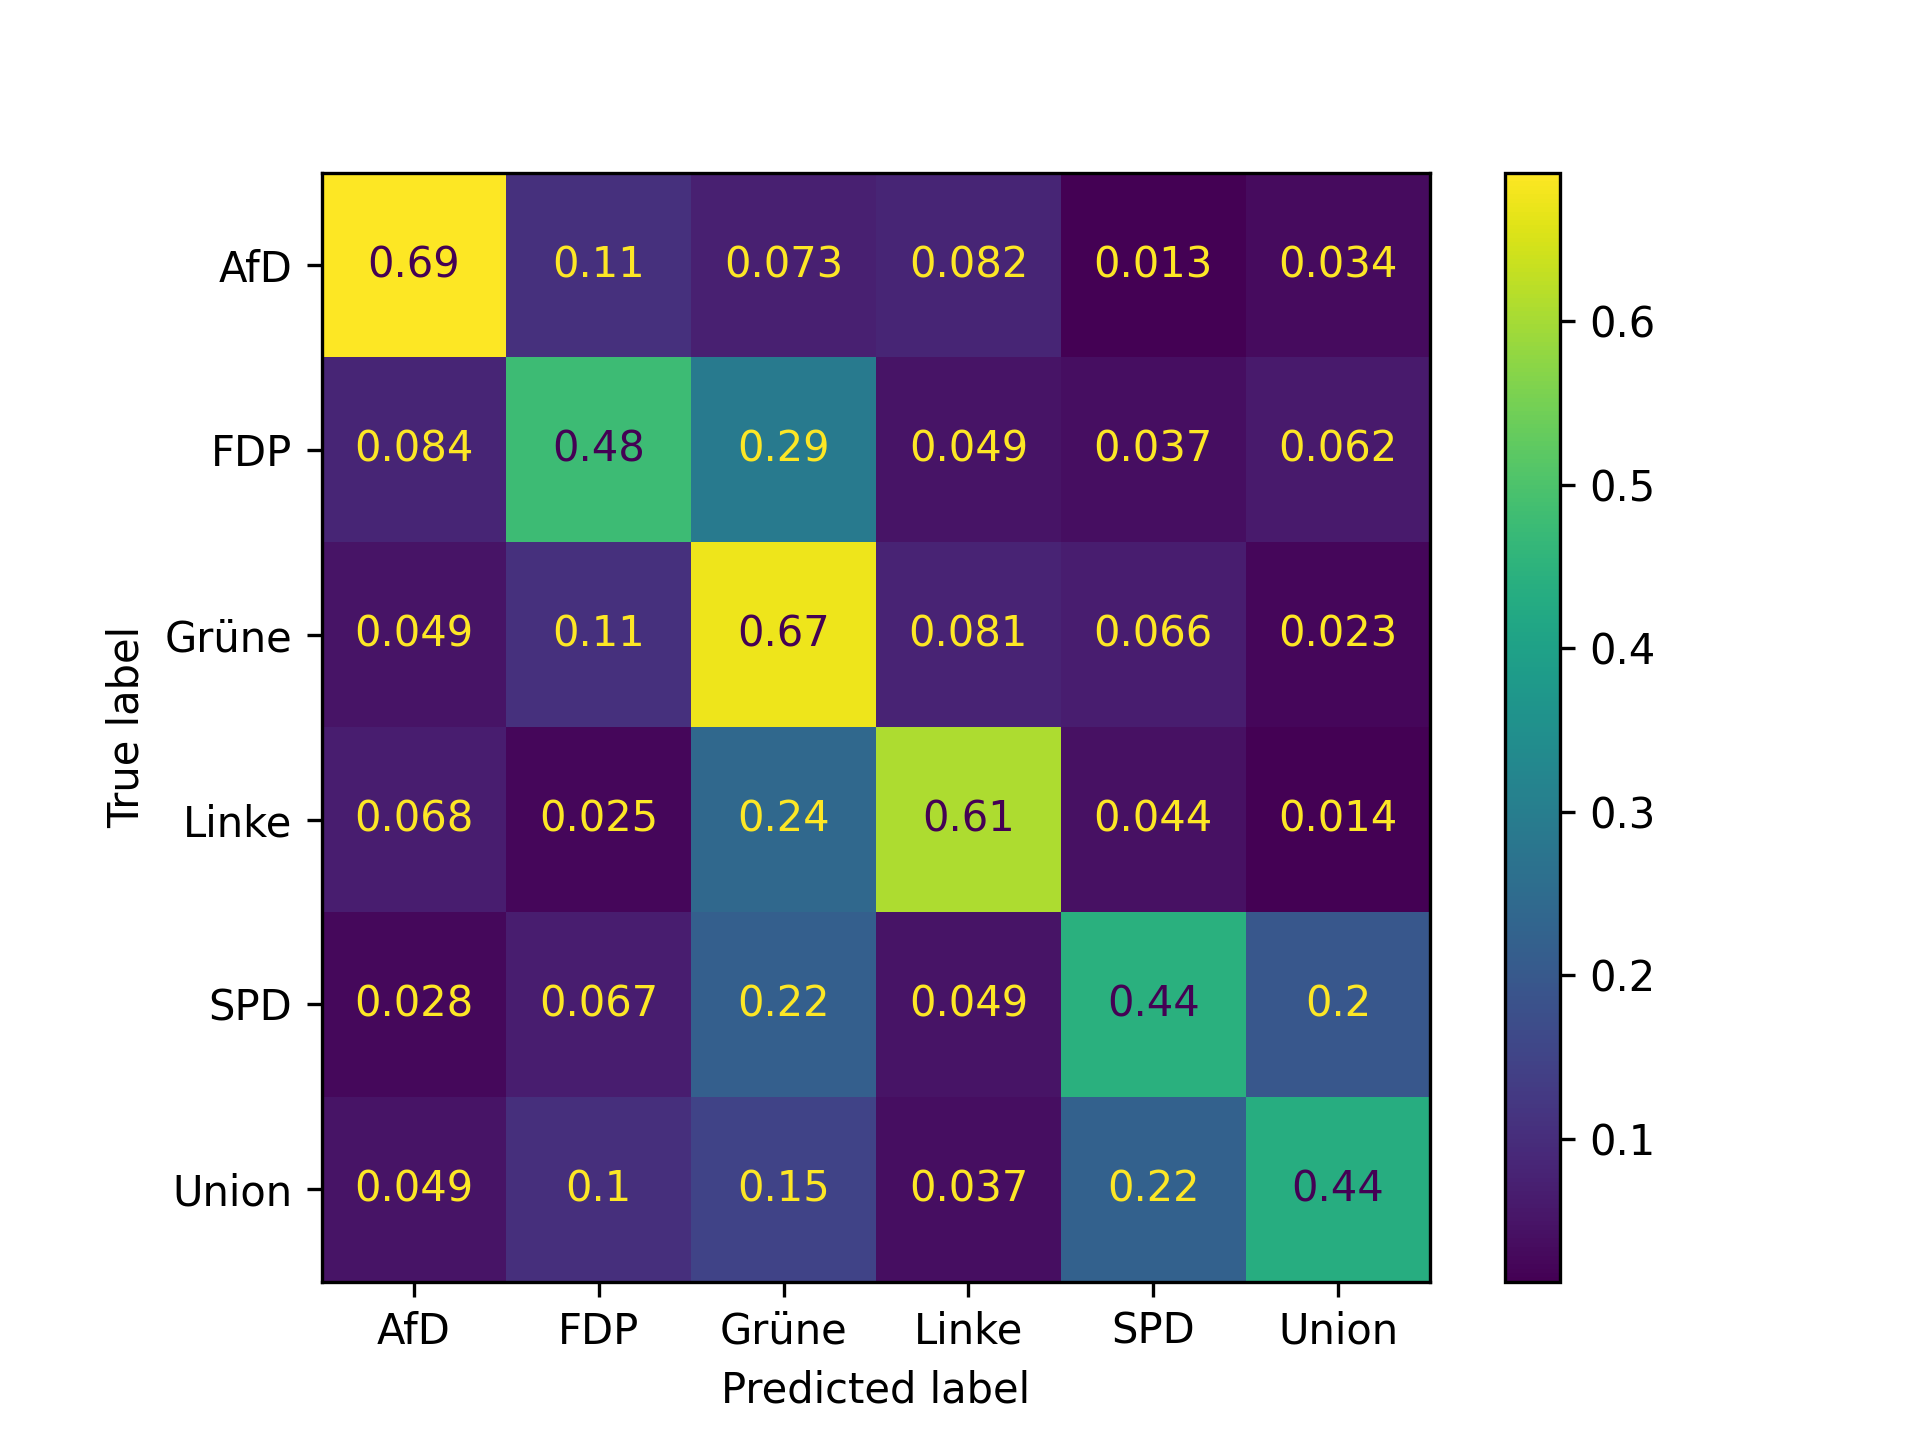
\includegraphics[width=\textwidth]{data/images/modeling/cnn/under/speeches_confusion_matrix.png}
        \caption{Reden}
        \label{sfig:confusionMatrixCnnSpeeches}
    \end{subfigure}
    \hfill
    \begin{subfigure}{0.49\textwidth}
        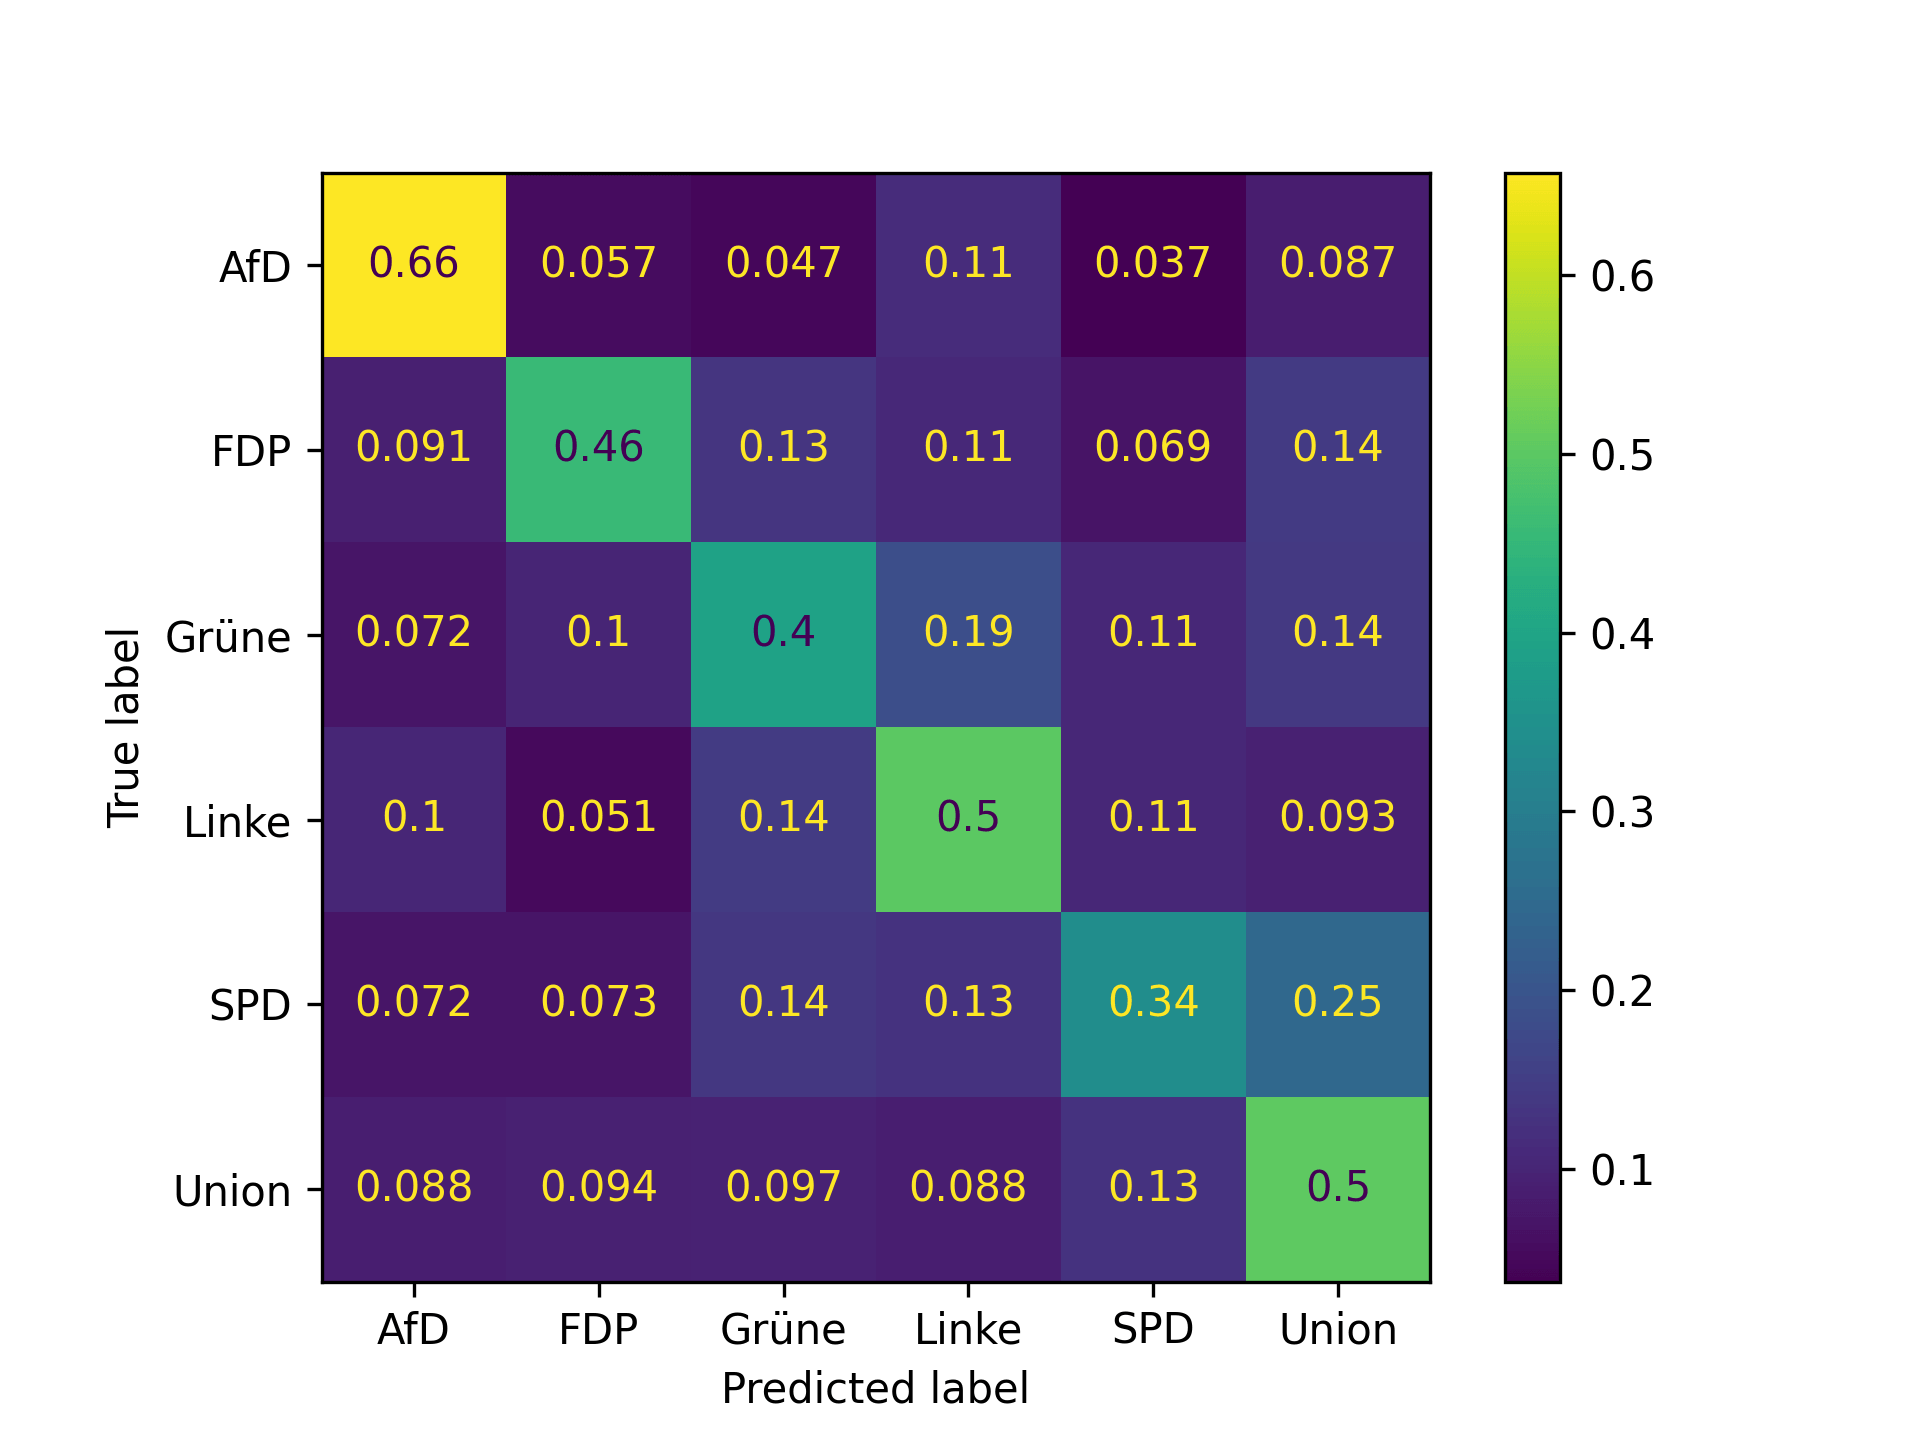
\includegraphics[width=\textwidth]{data/images/modeling/cnn/under/all_confusion_matrix.png}
        \caption{Kombiniert}
        \label{sfig:confusionMatrixCnnAll}
    \end{subfigure}
    \caption{Konfusionsmatrizen für das \acs{CNN}-Modell auf ausgeglichenen Datensätzen} \label{fig:confusionMatrixCnn}
\end{figure}

Die Konfusionsmatrix der Tweets in \autoref{sfig:confusionMatrixCnnTweets} zeigt, dass es zwischen bei den Parteien starke Unterschiede in der Falsch-Positiv-Rate gibt. Vor allem die Einträge der Grünen, als auch die der \ac{AfD} werden häufig falsch klassifiziert. Dabei lässt sich dieses Phänomen nicht auf einzelne Parteien reduzieren, da sich die falsch-positiven Werte auf jeweils alle anderen Parteien verteilen. Wie bereits bei den meisten Modellen und Datensätzen lassen sich auch hier hohe Falsch-Negativ-Raten zwischen \ac{SPD} und Union feststellen.

Wie \autoref{sfig:confusionMatrixCnnManifest} zeigt, weist das Modell einen starken Bias zur Union auf. Die Union verfügt zwar mit \SI{69}{\percent} über den höchsten Richtig-Positiv-Wert, zeigt aber gleichzeitig sehr viele falsch-positive Ergebnisse, vor allem zur \ac{SPD} mit \SI{39}{\percent} und zur \ac{FDP} mit \SI{29}{\percent}. Eine weitere Besonderheit bei den Wahlprogrammen ist die verhältnismäßig hohe gegenseitige Verwechslung zwischen \ac{AfD} und Linke von \SIrange{11}{13}{\percent}.

Bei den Reden, deren Konfusionsmatrix in \autoref{sfig:confusionMatrixCnnSpeeches} dargestellt ist, zeigt sich ein starker Bias zu den Grünen, die mit Abstand für die meisten falsch-positiven Vorhersagen sorgen. Dabei sind vor allem \ac{FDP}, Linke und \ac{SPD} betroffen, deren Reden als Grüne klassifiziert werden. Während auch \SI{15}{\percent} der Reden der Union als Grün klassifiziert werden, ist einzig die \ac{AfD} nur geringfügig von dem Bias zu den Grünen betroffen. Ferner ist -- wie im Ergebnis der meisten Trainings-Vorgänge -- eine starke Verwechslung innerhalb der beiden Koalitionsparteien Union und \ac{SPD} festzustellen.

Für das auf dem kombinierten Datensatz trainierte Modell (\autoref{sfig:confusionMatrixCnnAll}) fällt im Gegensatz zu den drei zuvor betrachteten Konfusionsmatrizen keine eindeutige Bias zu einer der Parteien auf. Viele Verwechslungen treten innerhalb der linken Parteien (Linke, Grüne und \ac{SPD}) auf. Zudem zeigt sich jeweils eine auffällige, symmetrische Vertauschung zwischen \ac{AfD} und Linken sowie zwischen Grünen und \ac{FDP}. Der Falsch-Negativ-Wert der \ac{SPD} zur Union ist mit \SI{25}{\percent} der höchste abseits der Richtig-Positiv-Achse.

\section{Bidirectional Encoder Representations from Transformers} \label{sec:trainingBert}

\ac{BERT} basiert auf der Transformer-Architektur und wurde \num{2018} von Google veröffentlicht \autocite{devlin_bert_2019}. DistilBERT ist eine Abwandelung von \ac{BERT}, die nahezu die gleiche Performance bei jedoch \SI{60}{\percent} weniger Ressourcenbedarf \autocite{sanh_distilbert_2020} bietet. In diesem Abschnitt werden die Ergebnisse für das Training mit beiden Modellen präsentiert. Für das Training werden die folgenden vortrainierten Modelle verwendet: \texttt{dbmdz/bert-base-german-uncased}\footnote{\href{https://huggingface.co/dbmdz/bert-base-german-uncased}{https://huggingface.co/dbmdz/bert-base-german-uncased}} (veröffentlicht unter MIT-Lizenz) und \texttt{distilbert-base-german-cased}\footnote{\href{https://huggingface.co/distilbert-base-german-cased}{https://huggingface.co/distilbert-base-german-cased}} (veröffentlicht unter Apache-Lizenz Version 2.0). Beide Modelle sind auf deutschen Datensätzen trainiert.

Für die Learning-Rate wird der gleiche Wert von \num{2e-5} wie bei \textcite{guhr_training_2020} angenommen. Die Batch-Size wird abhängig vom Datensatz und Modell variiert, um eine Balance zwischen Ressourcenbedarf und Trainingsgeschwindigkeit zu erreichen. Identisch zu \citeauthor{guhr_training_2020} werden beide Modelle für \num{3} Epochen trainiert. Wie bei dem \ac{CNN}-Ansatz wird lediglich mit den bereinigten, aber nicht tokenisierten Daten trainiert.

{\footnotesize
\begin{longtblr}[caption={Makro \(F_1\) Score für \acs{BERT} und DistilBERT}, label={tab:overviewScoresBert}, remark{Parameter} = {\(E = \num{3}\), \(LR = \num{2e-5}\), \(8 \leq B \leq 32\)}, note{$\dag$}={\ac{GDDR5} Speicher reicht nicht für das Training.}]{hline{1, 3, Y-Z} = {0.75pt}, rowhead = 2, colspec={l*{4}{Q[si={table-format=1.2},c]}}, row{1-2}={guard,font=\bfseries,l}}
     & \SetCell[c=2]{c} BERT & & \SetCell[c=2]{c} DistilBERT & \\ 
    \cline{2-5}
    Datensatz & Unbalanced & Balanced & Unbalanced & Balanced \\ 

    Tweets & \textbf{\num{0.62}} & 0.59 & 0.58 & 0.56 \\*
    Wahlprogramm & \textbf{\num{0.66}} & 0.61 & 0.62 & 0.58 \\*
    Reden & \textbf{\num{0.72}} & 0.66 & 0.67 & 0.65 \\*

    Kombiniert & \text{NA}\TblrNote{$\dag$} & \text{NA}\TblrNote{$\dag$} & \textbf{\num{0.60}} & 0.58 \\
\end{longtblr}
}

Aufgrund von der Komplexität von \ac{BERT} und DistilBERT benötigen beide Modelle mehr Zeit als die bisherigen Ansätze. Das Training des DistilBERT Modell benötigt zwischen \SIrange{10}{118}{\minute} abhängig vom Datensatz und ob Unterabtastung angewendet wird. Das \ac{BERT} Modell benötigt sogar zwischen \SIrange{24}{175}{\minute}, weil \ac{BERT} im Vergleich zu DistilBERT größer ist und zusätzliche Berechnungen durchführt \autocite{sanh_distilbert_2020}. Die Zeiten beinhalten ebenfalls die Zeit zum Speichern und Validieren nach jeder einzelnen Epoche. Neben der Laufzeit benötigt das \ac{BERT} Modell nahezu immer die vollen \SI{8}{\giga\byte} \ac{GDDR5} Speicher, wohingegen DistilBERT mit knapp der Hälfte auskommt.

Aus \autoref{tab:overviewScoresBert} geht hervor, dass das \ac{BERT} Modell grundsätzlich bessere Makro \(F_1\) Scores erreicht. Unabhängig vom Modell und ob Unterabtastung angewendet wurde, lassen sich die Reden am besten klassifizieren, gefolgt von den Wahlprogrammen. Am schlechtesten lassen sich Tweets klassifizieren. Wie zu erwarten scheidet \ac{BERT} in jeder Trainingskombination zwischen \numrange{0.01}{0.05} besser ab. Um \ac{BERT} auf dem kombinierten Datensatz trainieren zu lassen, werden mehr als \SI{8}{\giga\byte} \ac{GDDR5} Speicher benötigt. DistilBERT erreicht auf dem kombinierten Datensatz und den unbalancierten Daten einen Wert von \num{0.60} und \num{0.58} auf dem balancierten Datensatz.

\begin{figure}[H]
    \centering
    \begin{subfigure}{0.49\textwidth}
      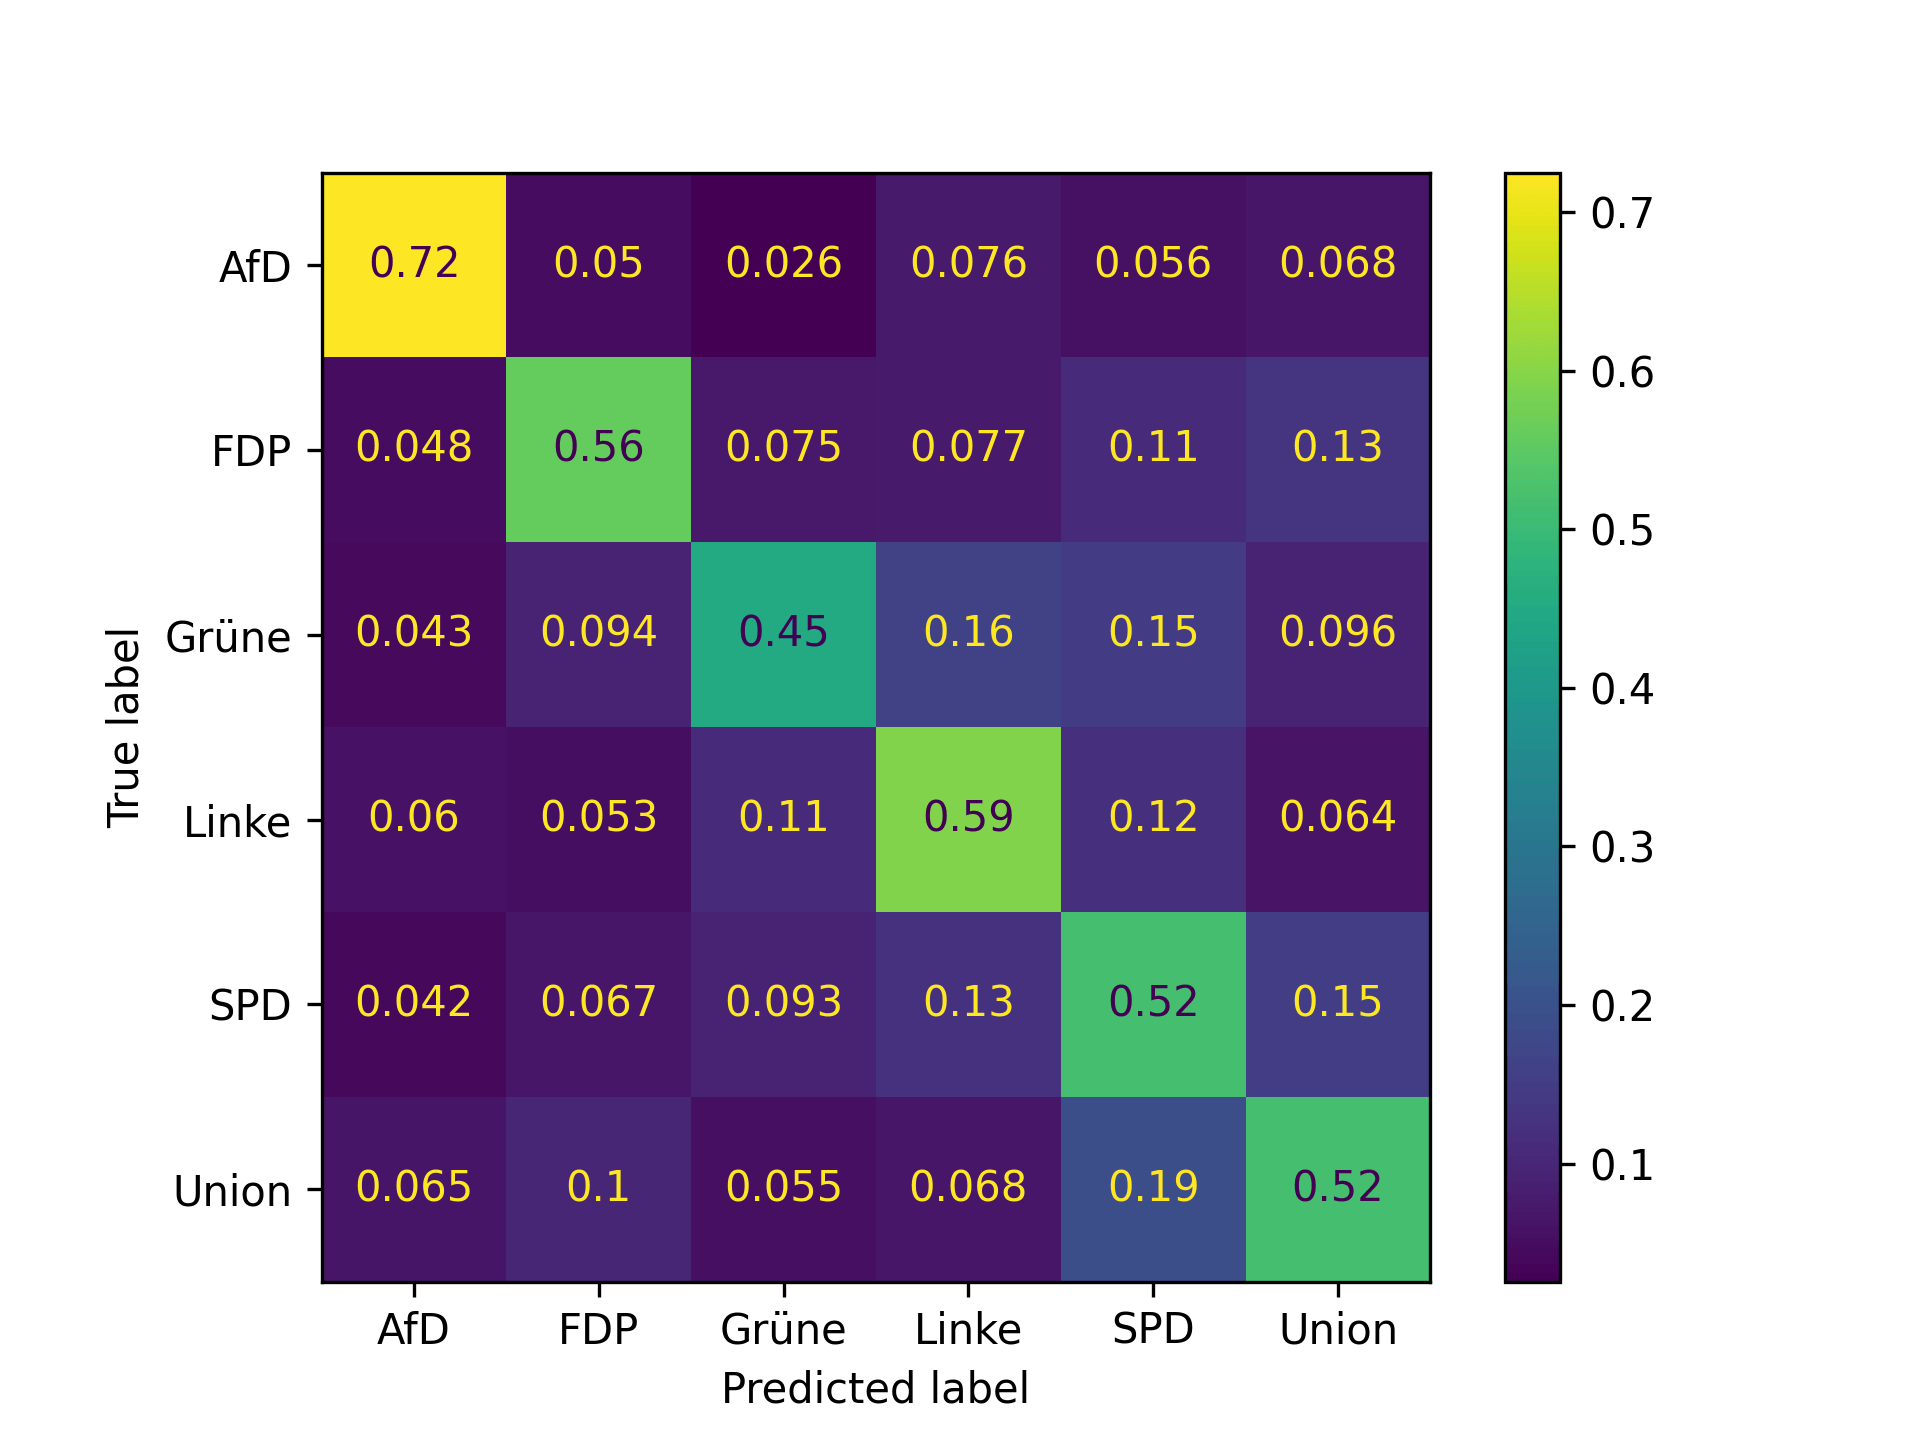
\includegraphics[width=\textwidth]{data/images/modeling/bert/under/tweets_confusion_matrix.png}
      \caption{Tweets} \label{sfig:confusionMatrixBertTweets}
    \end{subfigure}
    \hfill
    \begin{subfigure}{0.49\textwidth}
      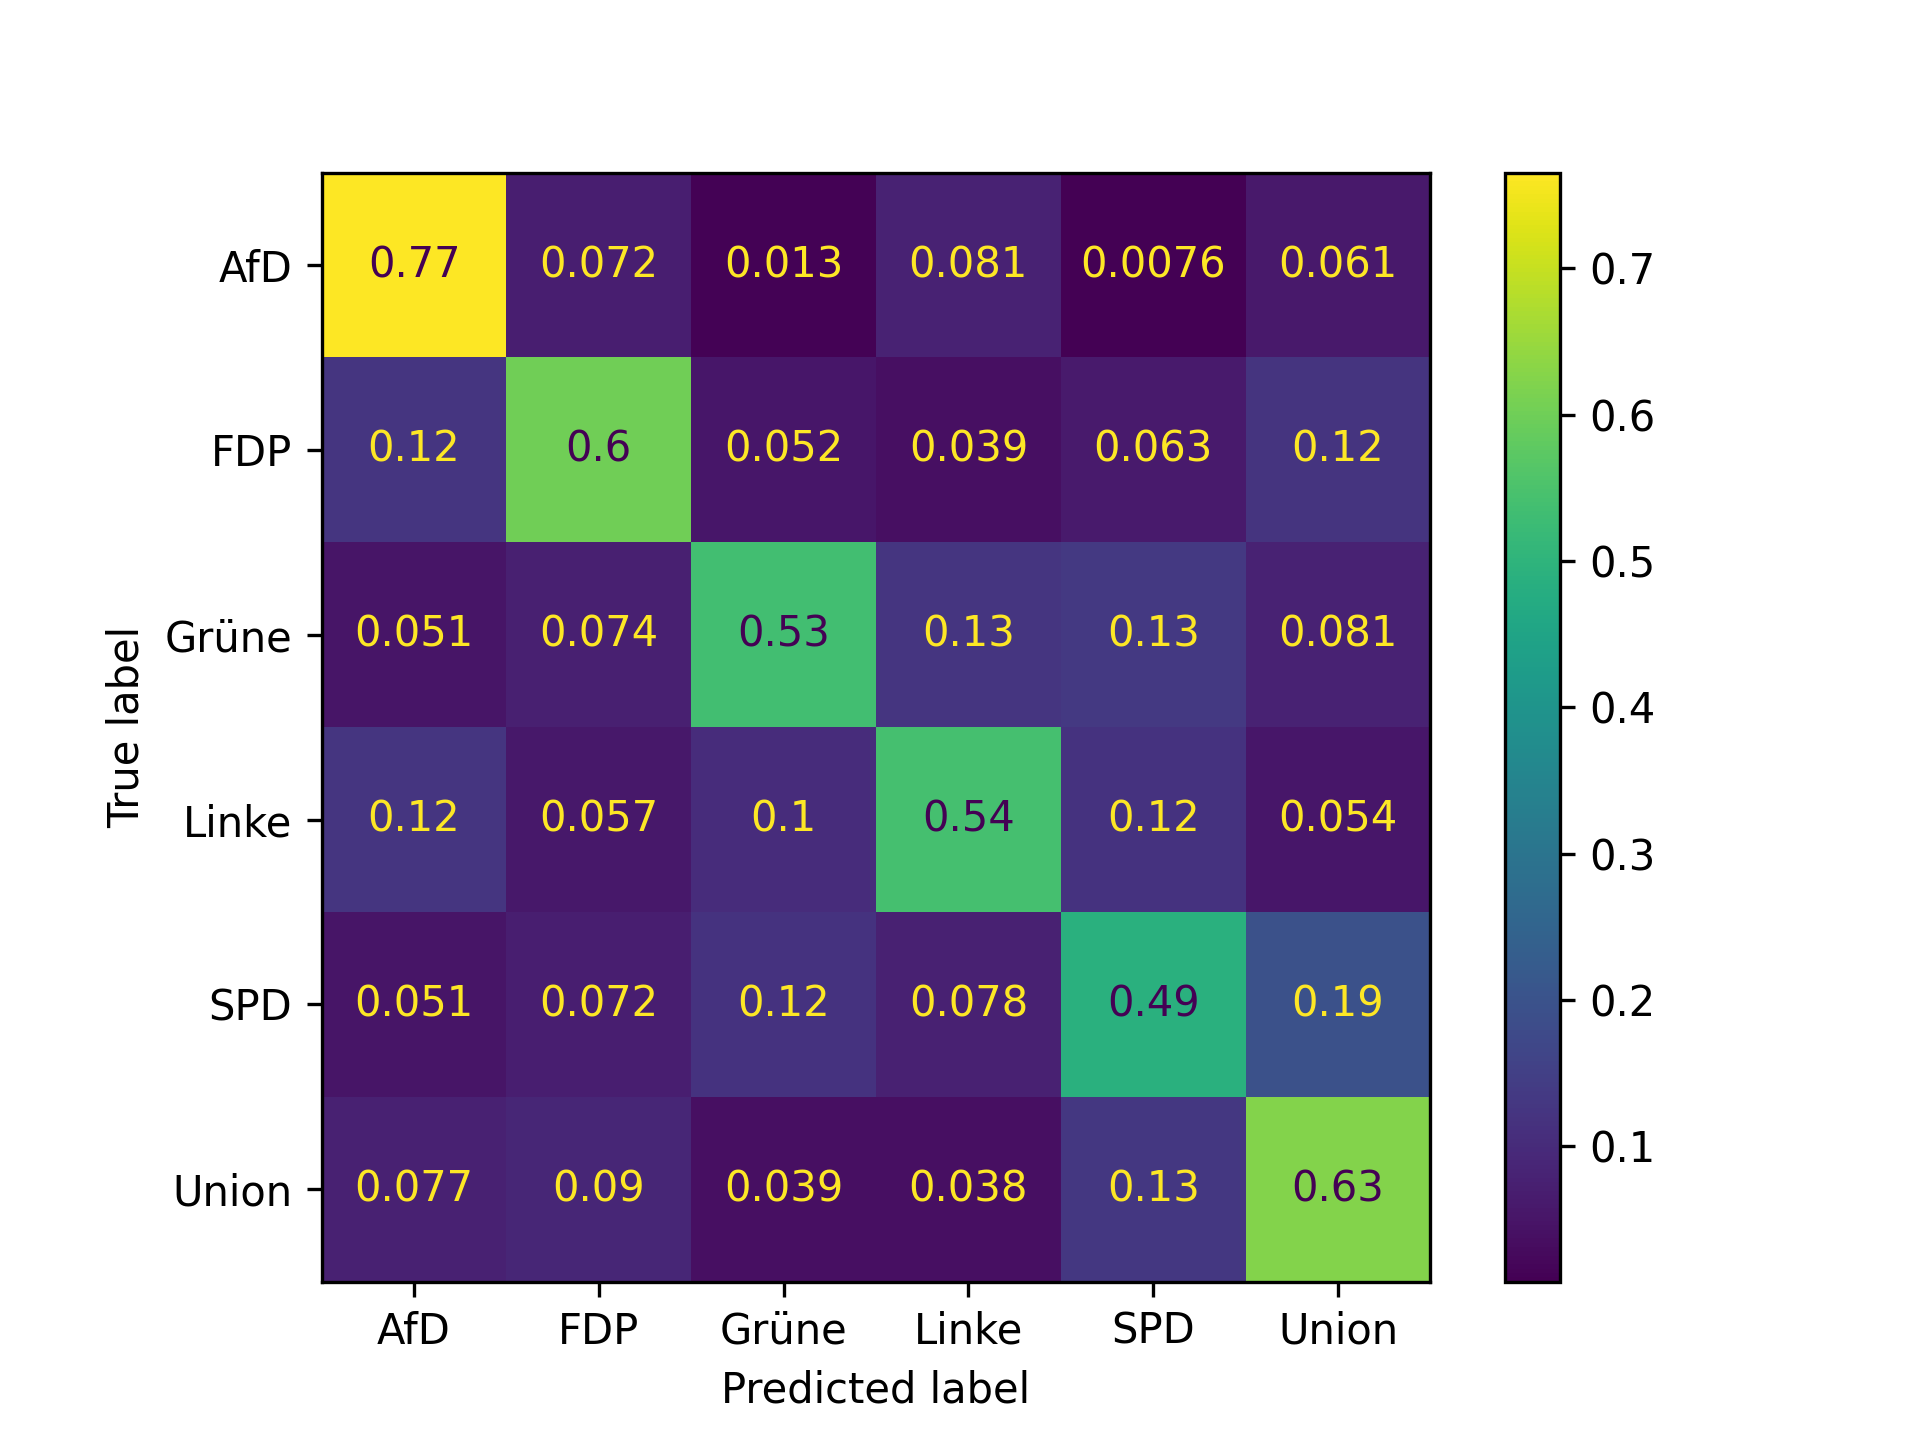
\includegraphics[width=\textwidth]{data/images/modeling/bert/under/party_programs_confusion_matrix.png}
      \caption{Wahlprogramme} \label{sfig:confusionMatrixBertManifest}
    \end{subfigure}
    \hfill
    \begin{subfigure}{0.49\textwidth}
      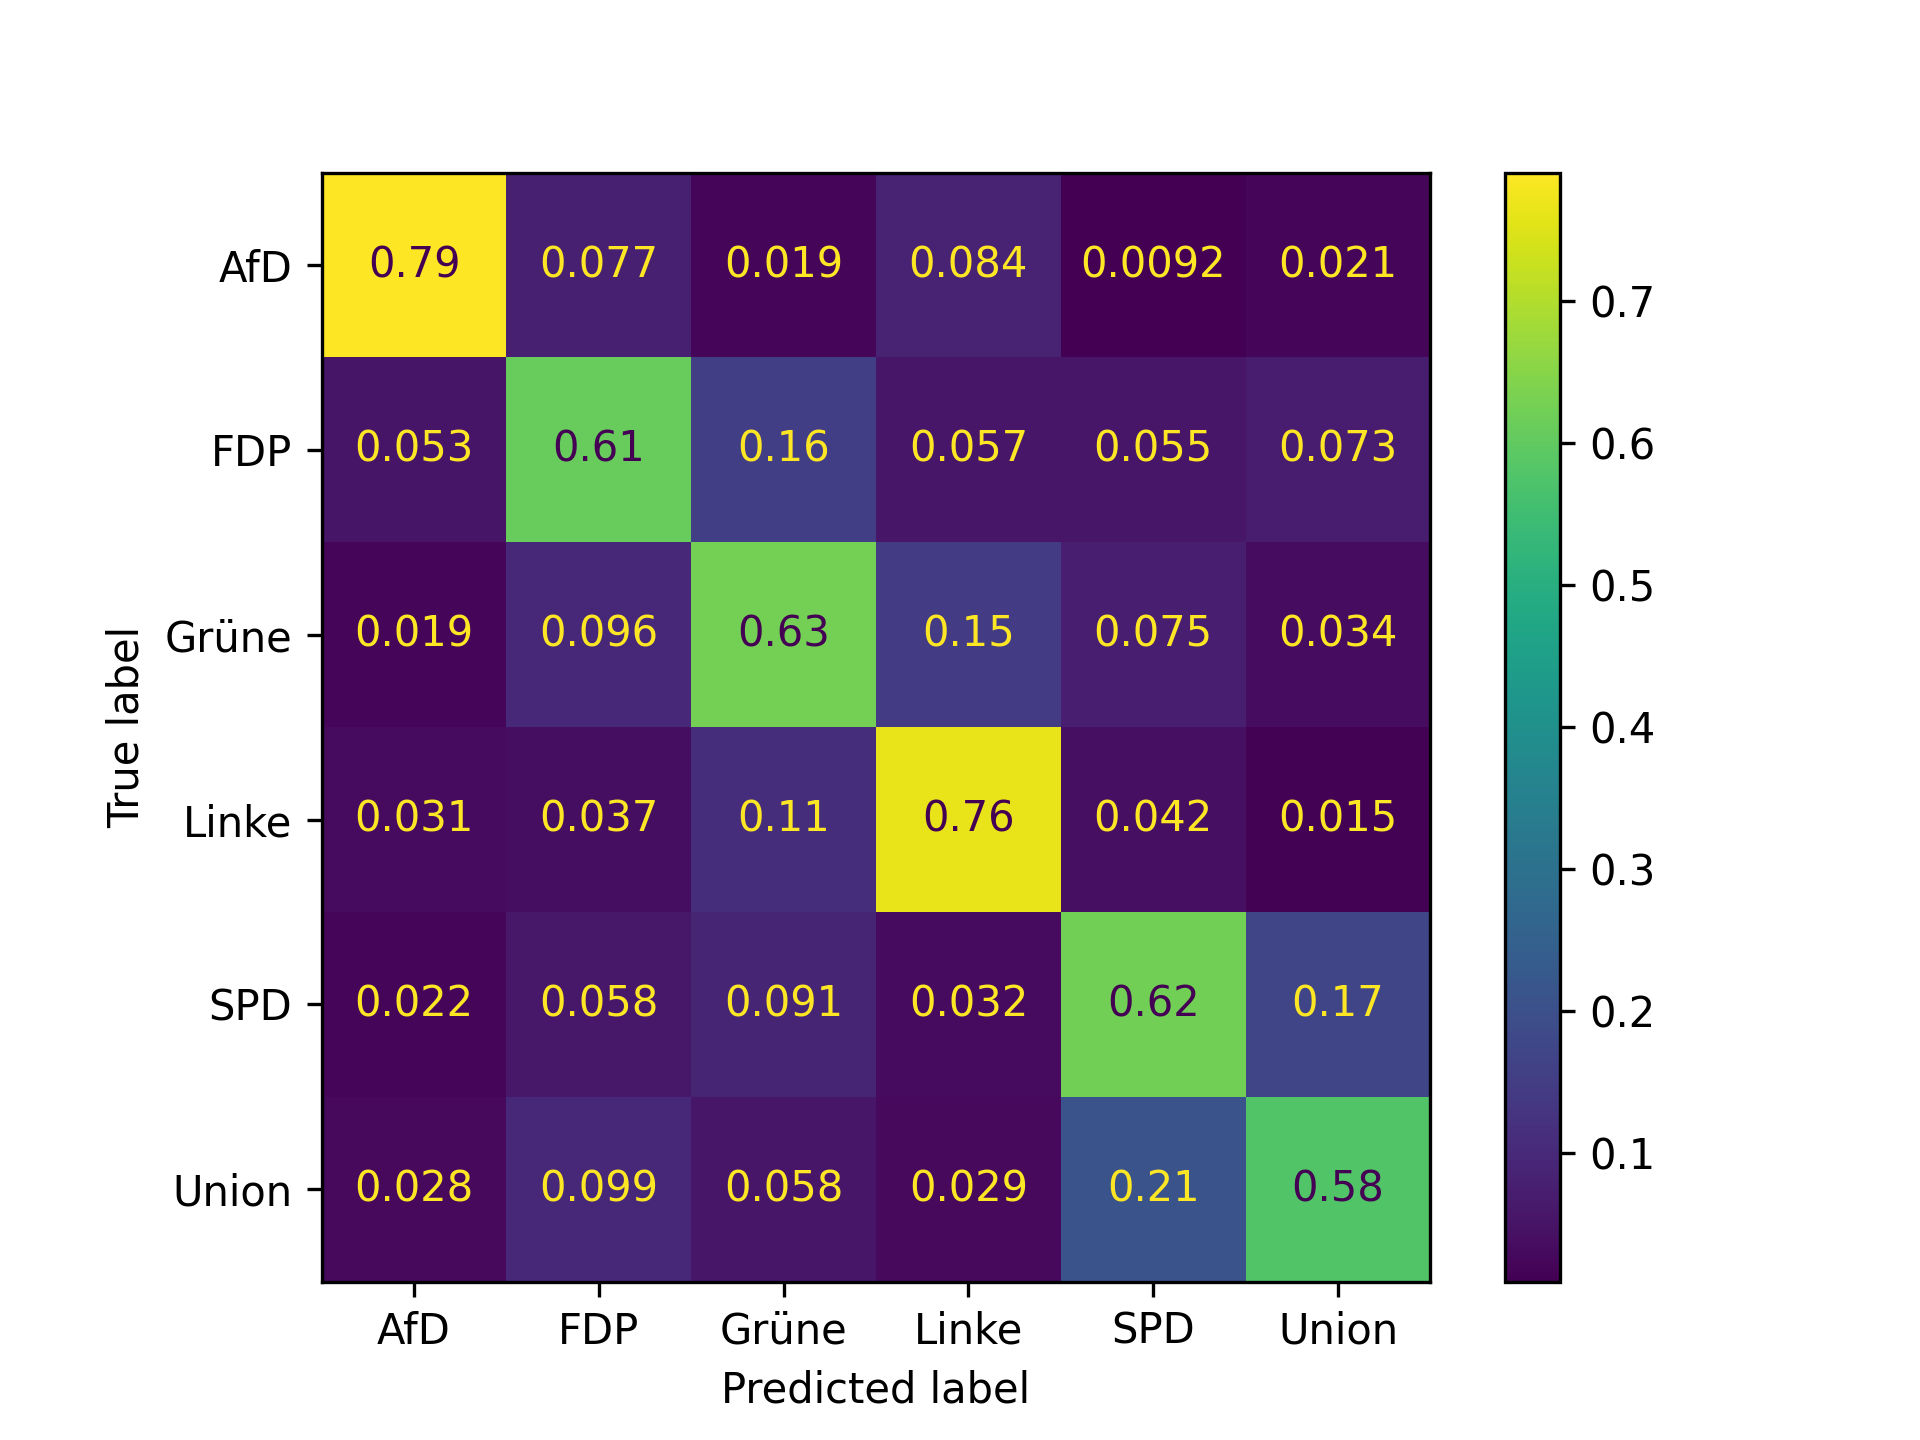
\includegraphics[width=\textwidth]{data/images/modeling/bert/under/speeches_confusion_matrix.png}
      \caption{Reden} \label{sfig:confusionMatrixBertSpeeches}
    \end{subfigure}
    \hfill
    \begin{subfigure}{0.49\textwidth}
      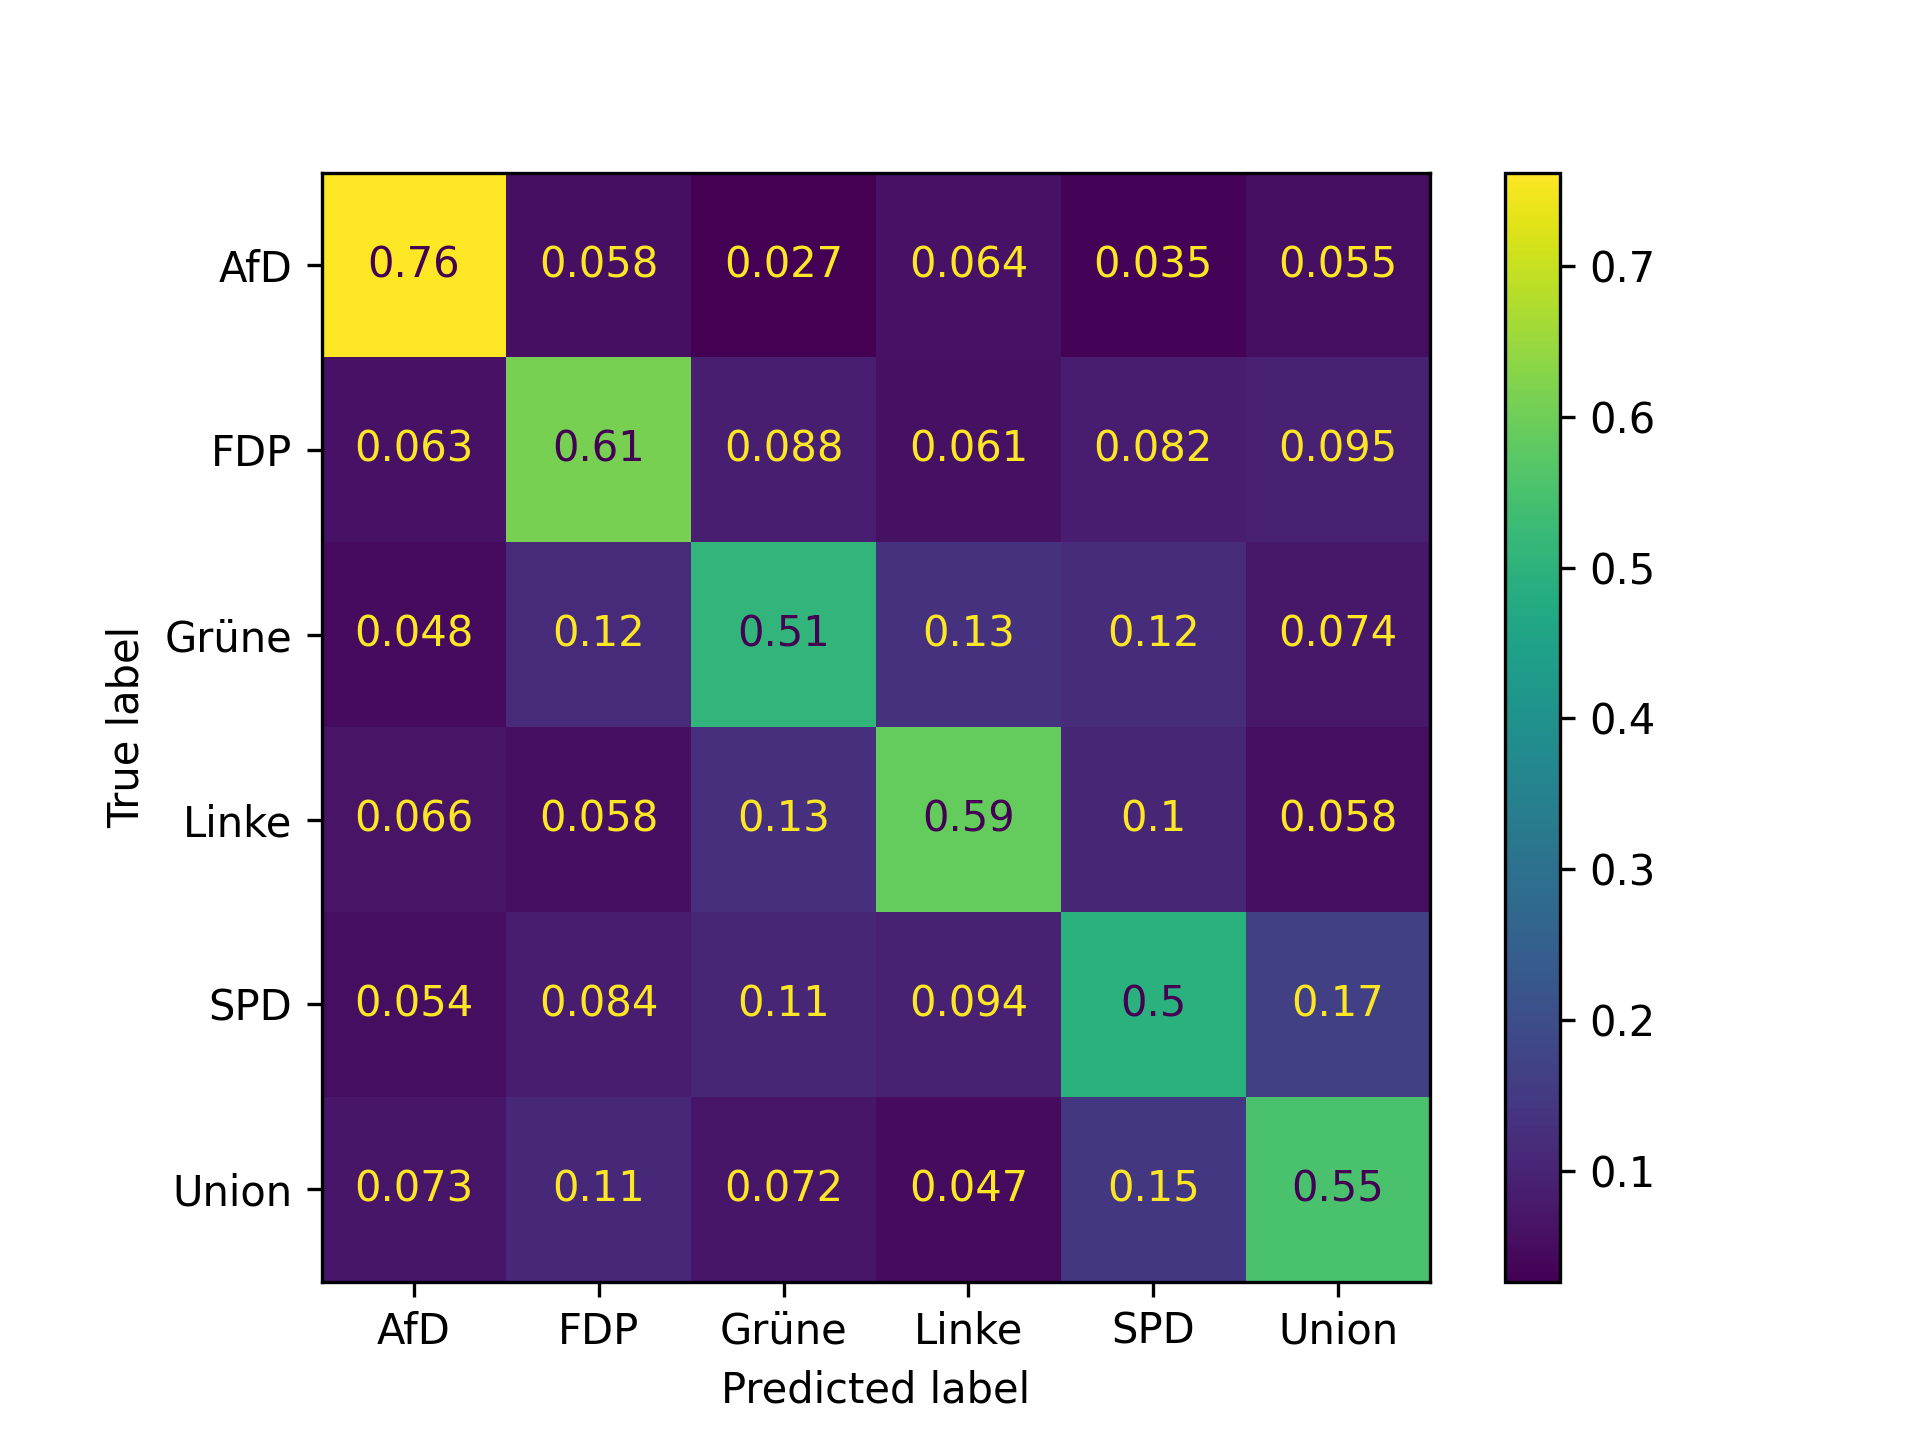
\includegraphics[width=\textwidth]{data/images/modeling/bert/under/all_confusion_matrix.png}
      \caption{Kombiniert} \label{sfig:confusionMatrixBertAll}
    \end{subfigure}
    \caption{Konfusionsmatrizen für DistilBERT auf ausgeglichenen Datensätzen} \label{fig:confusionMatrixDistilbert}
\end{figure}

Wie zuvor beschrieben, lässt sich \texttt{dbmdz/bert-base-german-uncased} aufgrund von mangelnden Ressourcen nicht auf dem gesamten Datensatz trainieren. Vergleicht man darüber hinaus DistilBERT auf den balancierten (\autoref{fig:confusionMatrixDistilbert}) und unbalancierten Daten (\autoref{fig:confusionMatrixDistilbertUnbalanced}), wird ersichtlich, dass das Modell auf den unbalancierten Daten einen starken Bias hin zur \ac{SPD} und Union besitzt. Dies lässt sich daran erklären, dass nach \autoref{tab:countPerDatasetAfterCleaning} beide Parteien mit am meisten Einträge besitzen. Aus den genannten Gründen wird das \texttt{distilbert-base-german-cased} Modell auf den balancierten Daten gewählt.

Die Konfusionsmatrix für DistilBERT (\autoref{fig:confusionMatrixDistilbert}) weist identische Muster zu den bisherigen Modellen auf. Zum einen zeigt sich eine große Verwechselung bei den linken Parteien. Ferner werden die beiden Regierungsparteien (\ac{SPD} und Union) mit \SIrange{13}{21}{\percent} häufig verwechselt. In Bezug auf die Klassifizierung der Reden lassen sich die Parteien \ac{AfD} und Linke mit deutlichem Abstand am besten differenzieren. Insbesondere jedoch zeigt sich erneut, dass die \ac{AfD} generell am besten klassifiziert werden kann. Die Analyse der kombinierten Daten verdeutlicht jedoch, dass die \ac{SPD} mit einer Genauigkeitsrate von lediglich \SI{50}{\percent} die schlechteste Klassifizierung aufweist. Die restlichen Parteien erzielen ebenfalls nur Werte zwischen \SIrange{51}{61}{\percent}.

Abschließend lässt sich festhalten, dass bei diesem Modell kein übermäßiger Bias festgestellt werden kann. Dennoch sollten die Ergebnisse mit Vorsicht betrachtet werden, da das Modell insgesamt keine optimale Leistung aufweist. Daher ist es ratsam, die Resultate mit kritischer Betrachtung zu interpretieren.

\section{Beobachtungen}

Die vorliegenden Ergebnisse verdeutlichen die Komplexität der Klassifizierung politischer Texte. Bei den Parteien mit ähnlichen politischen Idealen und nahe liegenden Themenschwerpunkten neigen die Modelle zu Verwechslungen. Dieses Phänomen ist insbesondere innerhalb der linken Parteien (Linke, \ac{SPD}, Grüne) sowie bei der \ac{FDP} und \ac{CDU} zu beobachten. Die \ac{AfD} hingegen bildet eine Ausnahme und lässt sich daher am besten klassifizieren.

Bei den untersuchten Modellen lassen sich aufgrund von Ressourcenbeschränkungen zwei der fünf Modelle (Baseline und \ac{MLP}, die beiden auf \ac{BoW} oder \ac{TF-IDF} basieren) nicht auf dem kombinierten Datensatz trainieren. Bei den BERT-Modellen ist dies sogar nur mit dem kleineren DistilBERT möglich. Auf dem kombinierten Datensatz erzielt DistilBERT den höchsten \(F_1\) Score auf den unausgeglichenen Daten, gefolgt von \ft mit einem geringfügigen Unterschied von \num{0.01}.

In Bezug auf die Trainingsdauer lassen sich die Modelle in zwei Lager einteilen. Die schnell trainierbaren Modelle wie Lineare \ac{SVC}, Multinomial \ac{NB}, \ft und \acp{CNN}, während \ac{MLP}, \ac{BERT} und DistilBERT zu den langsamer trainierbaren Modellen zählen.

Basierend auf der Genauigkeit, Trainingsdauer und Verteilung der Falsch-Negativ- und Falsch-Positiv-Raten lässt sich folgende wertende Reihenfolge ableiten: \ac{BERT} und DistilBERT erzielen die besten Ergebnisse, gefolgt von \ft. Lineare \ac{SVC} mit \ac{TF-IDF} erreicht ebenfalls gute Ergebnisse, muss jedoch aufgrund von Ressourcenbeschränkungen teilweise eingeschränkt werden. Die \ac{MLP}-Modelle zeigen ähnliche Einschränkungen aufgrund von Ressourcenmangel. Die \acp{CNN}-Modelle weisen eine hohe Streuung von Falsch-Positiv-Werten auf und erzielen inakkuratere Ergebnisse als die anderen Modelle.
